\documentclass[P]{BrJG_submit}  
%% Options:	[M] Manuscript format for submissions.
%%          [P] Paper format for testing.

%
%%%%%%%%%%%%%%%%%%%%%%%%%%%%%%%%
% 
\title{3D displacement and stress fields of compacting reservoir:  Alternative solutions}
\shorttitle{Compacting reservoirs}
%%%%%%%
%    O comando \affil serve para escrever os números referentes às filiações como sobrescritos após os 
%    nomes dos autores.
\author{Valeria C. F. Barbosa,\affil{1} Vanderlei C. Oliveira Jr,\affil{1}
Andre D. Arelaro\affil{1,2} and Filipe Borges\affil{2} }
\shortauthors{Barbosa et al.}
\correspondent{Valeria C. F. Barbosa}
%
\keywords{gravitational potential, reservoir compaction, hydrocarbon production, nucleus-of-strain solution,  mathematical and numerical modeling}

\ano{2022}

%

\begin{document}
%%%%%
%    The \affiliation command has two arguments: the affiliation number and the institution. Make sure that the affiliation
%    numbers correspond to those put in the  \affil commands.
%    The \affiliation commands must be placed immediately after \begin{document}.

%\affil{1}{Observat\'{o}rio Nacional, Rio de Janeiro, Brazil}
%\affil{2}{Petróleo Brasileiro S.A. (PETROBRAS), Rio de Janeiro, Brazil}

\affiliation{1}{Observat\'{o}rio Nacional, Rio de Janeiro, Brazil}
\affiliation{2}{Petróleo Brasileiro S.A. (PETROBRAS), Rio de Janeiro, Brazil}

%
\begin{abstract}
We have presented alternative solutions for the displacement and stress fields outside and inside of a 3D right rectangular prism  under constant pressure. These solutions are obtained by integrating the well-known nucleus-of-strain solution over the volume of the prism. They are based on the similarity between the gravitational potential yielded by a volume source under a density variation and the thermoelastic displacement potential yielded by a volume source in a half-space under a pressure variation. This similarity enables the use of closed expressions of the gravitational potential 
and its derivatives. We use our solution for approximating the displacement and stress fields
due to a reservoir with arbitrary shape and under arbitrary pressure changes.
We discretized the reservoir as a grid of 3D right rectangular prisms  juxtaposed in the horizontal and vertical directions. Each prism has homogeneous pressure; however, pressure variations among different prisms are allowed.  This parametrization of the reservoir yields a piecewise-constant distribution of pressure in the subsurface.  We validate the resultant displacement and stress fields due to the reservoir by numerical simulations including a reservoir with arbitrary geometry and under arbitrary pressure distribution, based on a production oil field in offshore Brazil.
\end{abstract}

\begin{resumo}
We have presented alternative solutions for the displacement and stress fields outside and inside of a 3D right rectangular prism  under constant pressure. These solutions are obtained by integrating the well-known nucleus-of-strain solution over the volume of the prism. They are based on the similarity between the gravitational potential yielded by a volume source under a density variation and the thermoelastic displacement potential yielded by a volume source in a half-space under a pressure variation. This similarity enables the use of closed expressions of the gravitational potential 
and its derivatives. We use our solution for approximating the displacement and stress fields
due to a reservoir with arbitrary shape and under arbitrary pressure changes.
We discretized the reservoir as a grid of 3D right rectangular prisms  juxtaposed in the horizontal and vertical directions. Each prism has homogeneous pressure; however, pressure variations among different prisms are allowed.  This parametrization of the reservoir yields a piecewise-constant distribution of pressure in the subsurface.  We validate the resultant displacement and stress fields due to the reservoir by numerical simulations including a reservoir with arbitrary geometry and under arbitrary pressure distribution, based on a production oil field in offshore Brazil.
\end{resumo}


\section*{Introduction}
The surface subsidence due to oil or gas withdrawal from a reservoir in the subsurface may occur as a result of geomechanical changes caused by pressure drop.
The phenomenon of subsidence by fluid extraction  has been observed in a variety of oil fields, e.g., the Ekofisk field, southern North Sea \citep{Borges2020} and the Groningen gas field in the northeast Netherlands \citep{vanThienenFokker17}.
Because the subsidence close to hydrocarbon fields under production can induce earthquakes (e.g., \citeauthor{Dahmetal15}, \citeyear{Dahmetal15}; \citeauthor{Grigolietal17}, \citeyear{Grigolietal17}), the petroleum companies  have been an increased interest in monitoring the magnitude and distribution of subsidence resulting from reservoir depletion.
This monitoring is accomplished by means of the numerical modeling of the displacement field.
The physical foundation of the displacement, stress and strain fields in the subsurface due to a reduction of pressure in the reservoir comes from the theory of thermoelasticity.
In the uncoupled thermoelasticity theory for quasi-static problems (i.e., problems with negligible inertia effects), \cite{Goodier37} employed the method of superposition using
displacement potential functions and introduced the  concept of nucleus of thermoelastic strain in an infinite space.
Specifically, Goodiee’s (\citeyear{Goodier37}) method simplified the thermoelastic problem by replacing it by an isothermal elastic problem with different boundary conditions together with the solution of a Poisson’s equation \citep{Tao71}. 
\cite{Mindlin-Cheng50} and \cite{Sen51} extended the Goodiee's method to a homogenous half-space.
\cite{Sharma56} deduced the displacement and stress fields in an infinite elastic plate due to a nucleus of thermoelastic strain located at a point inside it by using infinite integrals involving Bessel functions.

The subsidence resulting from reservoir depletion is in the context of poroelastic theory. 
\cite{Geertsma57} remarked the analogy between the theories of thermoelasticity and poroelasticity.
To our knowledge, \cite{Geertsma73} was the first to solve the poroelastic problem by using the nucleus-of-strain concept in the half-space, which in turn was proposed by \cite{Mindlin-Cheng50} and \cite{Sen51} in the theory of thermoelasticity.
Geertsma's approach presumes that the total displacement field due to the compaction of a
compacting region in subsurface is the superposition of the displacement field due to
its constituting points. 
Each constituting point, in turn, is represented by a small sphere called nucleus-of-strain. 
By using this idea, \cite{Geertsma73} derived analytical expressions by integrating the
nucleus-of-strain solution over the volume of a thin disk-shaped reservoir.
\cite{Segall92} followed \cite{Geertsma73} and extended the analytical solutions of the displacement and stress fields assuming general axisymmetric geometries and an arbitrary radial pressure distribution. 
\cite{Geertsma-Opstal73} applied the nucleus-of-strain concept in the half-space 
to calculate the spatial subsidence distribution due to the production of reservoir with an arbitrary 3D shape.
By assuming a producing reservoir embedded in an a homogeneous, isotropic, and elastic medium, and a reservoir model in which the pressure perturbations are related to the displacement field by a linear relationship, \cite{Geertsma-Opstal73} discretized the reservoir into a grid of  nuclei-of-strain and calculated the displacement due to the pressure change in the whole reservoir  by the superposition of the displacement due to the constant pressure change in each nucleus.
\cite{Tempone10} followed \cite{Geertsma-Opstal73} and 
extended the nucleus-of-strain concept in the half-space to consider the effects of a rigid basement. 
The main drawbacks in \cite{Geertsma-Opstal73} and \cite{Tempone10} are the assumption of homogeneous reservoir and the fact that the solution is only valid outside the reservoir.
In this case, the displacements within the reservoir are calculated by a linear interpolation of the displacements at the upper and lower edges of the reservoir \citep{Tempone12}.
Considering an inhomogeneous poroelastic model consists of layered stratigraphy, \cite{Mehrabian-Abousleiman15} developed closed-form formulae for the  displacement and stress  fields outside and inside of the reservoir embedded within elastic strata with different mechanical properties and subjected to pore pressure disturbances due to fluid extraction or injection. 
\cite{Munoz-Roehl17}  assume a linear elastic semi-infinite medium to develop an analytical solution for the  displacement field  outside and inside of a rectangular prism having a constant pressure change.
Their approach consists in integrating the Geertsma's nucleus-of-strain solution over the volume of the prism. Then, they discretize an arbitrarily-shaped reservoir under arbitrary distribution of pressure changes into a grid of  prisms having different constant pressure changes.
Finally, they compute the total displacement field outside and inside of the reservoir by adding the displacement fields produced by all prisms setting up the reservoir model.
 
The present work assumes a linear elastic semi-infinite medium and provides an alternative solution for the displacement field outside and inside of a rectangular prism with constant pressure change.
Like \cite{Munoz-Roehl17}, we integrate the Geertsma's nucleus-of-strain over the prism volume. 
We also use our alternative solution to approximate the displacement field due to an arbitrarily-shaped
reservoir under arbitrary pressures changes by the superposition of the displacement fields produced by
a grid of prisms.
Like \cite{Vasco1987}, we take advantage of the similarity between the  equations for calculating the displacement field due to a volume source in a half-space under a pressure variation and the gravitational potential due to a volume source under a density variation.
In contrast with \cite{Vasco1987}, our approach calculates the displacement field due to a 3D volume source
at the whole subsurface whereas \cite{Vasco1987} calculated the displacement field due to a 2D volume source
at the Earth surface.
We use closed expressions of the gravitational potential and its derivatives produced by the 3D right rectangular prism derived by \cite{Nagyetal2000}, \cite{Nagyetal2002}  and \cite{Fukushima2020}  for calculating the displacement field due to a 3D prism
under a constant pressure variation.
%\vspace{-0.5cm} 
\section*{Theory}
%\vspace{-0.5cm} 
The displacement, stress and strain fields in the subsurface caused by reservoir compactation due to hydrocarbon production are grounded on the theory of thermoelasticity. 
The Goodiee’s thermoelastic displacement potential $\phi$ satisfies the Poisson's equation \citep{Goodier37}, i.e.:
%\vspace{-1cm}
\begin{equation}
\nabla^{2} \phi =  m \: T,
\label{eq:poisson}
\end{equation}
where $\nabla^{2}$ is the Laplacian operator, $T $ is the temperature variation and 
$m =  \:  \alpha \: \frac{1 + \nu}{ 1 -\nu},$
%\begin{equation}
%m =  \:  \alpha \: \frac{1 + \nu}{ 1 -\nu},
%\label{eq:m}
%\end{equation}
where $\alpha$ is the coefficient of linear thermal expansion and $\nu$ is the Poisson's ratio.
From the potential theory, a particular solution of equation \ref{eq:poisson} is
%\vspace{-1cm}
\begin{equation}
\begin{aligned}
\phi(x,y,z) = & -  \frac{m}{4 \pi} \int\int\limits_{v}\int \\ 
   & \frac{T(x^{\prime}, y^{\prime}, z^{\prime} )}   
    {\sqrt{(x - x^{\prime})^{2} + (y - y^{\prime})^{2} + (z - z^{\prime})^{2}}} \: dv^{\prime},
\end{aligned}
\label{eq:phi}
\end{equation}
where $\phi(x,y,z)$ represents the Newtonian gravitational potential \citep{Kellogg29} that would be produced at the coordinates $x, y$ and $z$ by a continuous density distribution $- \frac{m}{4 \pi}  \: T( x^{\prime}, y^{\prime}, z^{\prime} )$. 
The integral in equation \ref{eq:phi} is conducted over the coordinates $x^{\prime}$,$y^{\prime}$ and $z^{\prime}$, denoting, respectively, the $x-$, $y-$ and $-z$ coordinates of an arbitrary point belonging to the interior of the volume $v$ of the solid. 
From equation \ref{eq:phi} and the potential theory, \citet{Goodier37} showed that, if an element of volume $dv$ in the infinite solid is at a temperature $T(x^{\prime}, y^{\prime}, z^{\prime}) $, the remainder being at temperature zero, the displacement vector $\bf{u}$ caused by this temperature is the gradient of the Goodiee’s thermoelastic displacement potential, i.e.,
%\vspace{-1cm}
\begin{equation}
{\bf{u}} = {\bf {\nabla}} \phi(x,y,z) \: ,
\label{eq:displacement-general}
\end{equation}
where $\bf{\nabla}$ is the gradient operator.  
To a homogenous half-space, \citet{Mindlin-Cheng50} showed that the method proposed by  \citet{Goodier37} can be extended by the displacement solution given by:
%\vspace{-1cm}
\begin{equation}
\bf{u} = {\bf{\nabla}} \: \phi_{1} \: + \: {\bf{{\nabla}_{2}}} \phi_{2}, 
\label{eq:displacement-solution}
\end{equation}
where $\phi_{1} \equiv \phi_{1}(x,y,z)$ is the potential defined in equation \ref{eq:phi}, 
$\phi_{2} \equiv  \phi_{2}(x,y,z)$
is defined as "image potential" \citep{Segall92} due to a image point at the coordinates
$(x^{\prime}, y^{\prime}, -z^{\prime} )$ and the operator $\bf{{\nabla}_{2}}$ is
%\vspace{-1cm}
\begin{equation}
{\bf{{\nabla}_{2}}} = (3 - 4\nu){\bf{\nabla}} + 2 {\bf{\nabla}} z \frac{\partial }{\partial z}  - 4(1- \nu){\bf{\hat{z}}} {\bf{{\nabla}^{2}_{z}}},
\label{eq:nabla2}
\end{equation}
where ${\bf{\hat{z}}}$ is the unit vector in the $z-$direction and 
${\bf{{\nabla}^{2}_{z}}}$ is a scalar operator in which the operand is firstly
multiplied by $z$ and then operated upon by the Laplacian ${\bf{\nabla}^{2}}$. 
Equation \ref{eq:displacement-solution} is the displacement solution for the variation of temperature due to a single nucleus of strain buried at depth $z^{\prime}$ in a
semi-infinite homogeneous medium. 
In the right hand side of equation \ref{eq:displacement-solution}, the first term 
$ {\bf{\nabla}} \: \phi_{1} $ represents the displacement in an infinite medium, and the second term represents a correction of the displacement due a half-space, also known as "image nucleus solution".

\section*{Methodology}
%\vspace{-1.0cm}
Let's assume that a reservoir in the interior of the Earth is subject to a compactation due to hydrocarbon production. 
The compactation is caused by the pressure change within the reservoir, which in turn causes  a surface subsidence (or surface displacement). 
Here, we use a Cartesian coordinate system with the $x-$axis pointing to north, the $y-$axis pointing to east and the $z-$axis pointing downward.
We discretize the reservoir into an $ m_{x} \times m_{y} \times m_{z} $ grid of 3D vertical juxtaposed prisms $(m_{x} \cdot m_{y} \cdot m_{z} = M)$ along the 
$x$, $y$ and $z$ axes, respectively, in which the pressure within each prism is 
assumed to be constant and known. 
Each prism in the reservoir model may undergo a distinct pressure change.
The subsidence effect is the displacement field due to the pressure change throughout the reservoir and is calculated by the sum of the displacement produced by each prism.
The discrete forward modeling to calculate the displacement and stress fields due to a piecewise-constant distribution of the pressure variation within a reservoir follows the nucleus-of-strain approach. 
We assume that a nucleus of strain represents an infinitesimal reservoir volume 
element. The displacement solution for a single nucleus of strain in a homogeneous elastic semi-infinite medium (equation \ref{eq:displacement-solution}) will be used as an element of the displacement.
We calculate the displacement (stress) field due to the pressure variation of a prism by integrating the nucleus of strain over its volume. 

\noindent{\textbf{The discrete forward modeling due to a nucleus of strain in a homogeneous elastic semi-infinite medium}}
%======================================================================================
%\subsection*{The discrete forward modeling due to a nucleus of strain %in a homogeneous elastic semi-infinite medium}\label{solution-nucleus}
%======================================================================================

By considering the discrete form of equation \ref{eq:displacement-solution}, the displacement vector  $ {\bf{u}}_{ij} \equiv  {\bf{u}}(x_{i}, y_{i}, z_{i}, x^{\prime}_{j}, y^{\prime}_{j}, z^{\prime}_{j})$ at an arbitrary point $(x_{i}, y_{i}, z_{i})$ due to a change of pressure in the $j$th nucleus of strain at the coordinates $(x^{\prime}_{j}, y^{\prime}_{j}, z^{\prime}_{j})$ will be calculated by
%\vspace{-1cm}
\begin{equation}
{\bf{u}}_{ij}  = {\bf{u_{1}}}_{ij} + {\bf{u_{2}}}_{ij} \: ,
\label{eq:displacement_ui}
\end{equation}
where ${\bf{u_{1}}}_{ij}$ is the displacement vector at the point $(x_{i}, y_{i}, z_{i})$ due to the $j$th single nucleus in the infinite space and ${\bf{u_{2}}}_{ij}$ 
is the correction of the displacement considering a semi-space (image nucleus solution).
The term ${\bf{u_{1}}}_{ij}$ (equation \ref{eq:displacement_ui}) is given by
%\vspace{-1cm}
\begin{equation}
{\bf{u_{1}}}_{ij} = A_{E} \: {\bf{\nabla}} \bigg( {\frac{1}{{R_1}_{ij}}} \bigg) 
\: \Delta p_{j} \: \:dv_j^{\prime}
\label{eq:nucleus-u1}
\end{equation}
and represents the gradient of the potential
%\vspace{-1cm}
\begin{equation}
\phi_{1} = - \frac{C_m}{4 \pi}  \frac{\Delta p_{j} \: \:dv_j^{\prime}}{ {R_1}_{ij} } \: .
\label{eq:nucleus-phi1}
\end{equation}
The term ${\bf{u_{2}}}_{ij}$ (equation \ref{eq:displacement_ui}) is given by
%\vspace{-1cm}
\begin{equation}
\begin{aligned}
{\bf{u_{2}}}_{ij} \!=  & 
A_{E} \!
\bigg[ 
C_{\nu} \: {\bf{\nabla}} \bigg(  {\frac{1}{{R_2}_{ij}}} \bigg)     
\! + 2 {\bf{\nabla}} \bigg( \! z \frac{\partial }{\partial z} {\frac{1}{{R_2}_{ij}}} \bigg) \\  
& - 4(1- \nu){\bf{\hat{z}}} {\bf{{\nabla}^{2}}}  \bigg(\! {\frac{z}{{R_2}_{ij}}} \bigg)
\bigg] \! \Delta p_{j}  dv_j^{\prime}
\end{aligned}
\label{eq:nucleus-u2}
\end{equation}
and is obtained by applying the operator ${\bf{{\nabla}_{2}}}$ (equation 
\ref{eq:nabla2}) to the image potential
%\vspace{-1cm}
\begin{equation}
\phi_{2} = - \frac{C_m}{4 \pi}  \frac{\Delta p_{j} \: \:dv_j^{\prime}}{ {R_2}_{ij} } \: .
\label{eq:nucleus-phi2}
\end{equation}
In equations \ref{eq:nucleus-u1}--\ref{eq:nucleus-phi2}, 
all derivatives are computed with respect to the coordinates of the point 
$(x_{i}, y_{i}, z_{i})$, 
$\Delta p_j$  is the pressure change of the $j$th nucleus, $dv_j^{\prime}$ is an 
infinitesimal element of volume centered at the $j$th nucleus of strain 
$(x^{\prime}_{j}, y^{\prime}_{j}, z^{\prime}_{j})$, 
$C_{\nu} = (3  -  4\nu)$, 
$A_{E} = \frac{A (1 + \nu)}{E}$,
where $A$ is the constant
%\vspace{-1cm}
\begin{equation}
A = - \frac{C_m E}{4 \pi (1 + \nu)} \: ,
\label{eq:nucleus-A}
\end{equation}
$E$ is the Young’s modulus and $C_m$ is the uniaxial compaction coefficient (see \citeauthor{Geertsma66}, 
\citeyear{Geertsma66}) 
%\vspace{-1cm}
\begin{equation}
C_m = \frac{1}{E} \: \frac{(1 + \nu) (1  - 2\nu)}{(1-\nu)} \: .
\label{eq:Cm}
\end{equation}
In equation \ref{eq:nucleus-phi1}, $ {R_1}_{ij}$ is the distance from the $i$th point $ (x_{i}, y_{i}, z_{i})$ to the $j$th nucleus of strain $(x^{\prime}_{j}, y^{\prime}_{j}, z^{\prime}_{j})$, i.e.:
${R_1}_{ij} = {\sqrt{(x_{i}- x^{\prime}_{j})^{2} + (y_{i} - y^{\prime}_{j})^{2} + 
(z_{i} - z^{\prime}_{j})^{2}}}.$
%\begin{equation}
%{R_1}_{ij} = {\sqrt{(x_{i}- x^{\prime}_{j})^{2} + (y_{i} - y^{\prime}_{j})^{2} + 
%(z_{i} - z^{\prime}_{j})^{2}}}.
%\label{eq:R1}
%\end{equation}
In equation \ref{eq:nucleus-phi2}, $ {R_2}_{ij}$ is the distance from the $i$th point $ (x_{i}, y_{i}, z_{i})$ to the $j$th image nucleus $(x^{\prime}_{j}, y^{\prime}_{j}, - z^{\prime}_{j})$, i.e.:
${R_2}_{ij} = {\sqrt{(x_{i}- x^{\prime}_{j})^{2} + (y_{i} - y^{\prime}_{j})^{2} + 
(z_{i} + z^{\prime}_{j})^{2}}}.$
%\begin{equation}
%{R_2}_{ij} = {\sqrt{(x_{i}- x^{\prime}_{j})^{2} + (y_{i} - y^{\prime}_{j})^{2} + 
%(z_{i} + z^{\prime}_{j})^{2}}} \: .
%\label{eq:R2}
%\end{equation}
Figure \ref{fig:nucleus_strain} shows a schematic representation of the geometry of the nucleus of strain problem in a semi-infinite medium. 
The horizontal plane $z = 0$ is called "free surface".
The $x-$, $y-$ and $z-$components of the vectors ${\bf{u_{1}}}_{ij}$ (equation \ref{eq:nucleus-u1}) and ${\bf{u_{2}}}_{ij}$ (equation \ref{eq:nucleus-u2}) can be explicitly defined as follows:
\begin{equation}
{\bf{u_{1}}}_{ij} = A_{E}
\begin{bmatrix} 
\frac{\partial }{\partial x} {\frac{1}{{R_1}_{ij}}}  \\
\frac{\partial }{\partial y} {\frac{1}{{R_1}_{ij}}}  \\
\frac{\partial }{\partial z} {\frac{1}{{R_1}_{ij}}} 
\end{bmatrix}
  \Delta p_{j} \:dv_j^{\prime}
\label{eq:nucleus-u1-vector}
\end{equation}
and 
%\vspace{-1cm}
\begin{equation}
{\bf{u_{2}}}_{ij} \! = \! 
A_{E} \! \left\{\! C_{\nu} \!
\begin{bmatrix} 
   \frac{\partial}{\partial x} {\frac{1}{{R_2}_{ij}}}  \\
   \frac{\partial}{\partial y} {\frac{1}{{R_2}_{ij}}}  \\
  -\frac{\partial}{\partial z} {\frac{1}{{R_2}_{ij}}}  
\end{bmatrix}
\! + \! 2 z_{i} \!
\begin{bmatrix} 
\frac{\partial^{2}}{\partial x \partial z} {\frac{1}{{R_2}_{ij}}} \\
\frac{\partial^{2}}{\partial y \partial z} {\frac{1}{{R_2}_{ij}}} \\
\frac{\partial^{2}}{\partial z^{2}} {\frac{1}{{R_2}_{ij}}} 
\end{bmatrix} \!
\right\} \! \!
\Delta p_{j} dv_j^{\prime}.
\label{eq:nucleus-u2-vector}
\end{equation}
By following \cite{Sharma56} and \cite{Tempone10}, 
the stress vector 
$\mbox{\boldmath$\sigma$}_{ij} \equiv \mbox{\boldmath$\sigma$}(x_{i}, y_{i}, z_{i}, x^{\prime}_{j}, y^{\prime}_{j}, z^{\prime}_{j})$ 
at the point $(x_{i}, y_{i}, z_{i})$ due to the $j$th single nucleus of strain buried 
in the half space is given by
%\vspace{-1cm}
\begin{equation}
\mbox{\boldmath$\sigma$}_{ij} = \mbox{\boldmath$\sigma_{1}$}_{ij} + 
\mbox{\boldmath$\sigma_{2}$}_{ij} \: ,
\label{eq:stress_nucleus}
\end{equation}
where $\mbox{\boldmath$\sigma_{1}$}_{ij} \equiv \mbox{\boldmath$\sigma_{1}$}(x_{i}, y_{i}, z_{i}, x^{\prime}_{j}, y^{\prime}_{j}, z^{\prime}_{j})$ is the stress vector 
at the point $(x_{i}, y_{i}, z_{i})$ due to the $j$th single nucleus in the infinite space and $\mbox{\boldmath$\sigma_{2}$}_{ij} \equiv \mbox{\boldmath$\sigma_{2}$}(x_{i}, y_{i}, z_{i}, x^{\prime}_{j}, y^{\prime}_{j}, z^{\prime}_{j})$ is the stress vector 
at the point $(x_{i}, y_{i}, z_{i})$ that gives the correction of the stress due to the 
$j$th image nucleus considering a semi-space. These two vectors are given by
\begin{equation}
\mbox{\boldmath$\sigma_{1}$}_{ij} =
A  \! 
\begin{bmatrix} 
\frac{\partial^{2} }{\partial x \partial z} {\frac{1}{{R_1}_{ij}}}  \\
\frac{\partial^{2} }{\partial y \partial z} {\frac{1}{{R_1}_{ij}}}  \\
\frac{\partial^{2} }{\partial z^{2}} {\frac{1}{{R_1}_{ij}}} 
\end{bmatrix}
\Delta p_{j} dv_j^{\prime},
\label{eq:nucleus-stress1-vector}
\end{equation}
%\vspace{-0.5cm}
and 
\begin{equation}
\mbox{\boldmath$\sigma_{2}$}_{ij} = \! 
A  \! 
\left\{
\begin{bmatrix} 
\frac{\partial^{2}  }{\partial x \partial z} {\frac{1}{{R_2}_{ij}}} \\
\frac{\partial^{2} }{\partial y \partial z} {\frac{1}{{R_2}_{ij}}} \\
- \frac{\partial^{2} }{\partial z^{2}} {\frac{1}{{R_2}_{ij}}}   
\end{bmatrix}
\! + \! 2 z_{i} \! 
\begin{bmatrix} 
\frac{\partial^{3}  }{\partial x \partial z^{2}} {\frac{1}{{R_2}_{ij}}} \\
\frac{\partial^{3} }{\partial y \partial z^{2}} {\frac{1}{{R_2}_{ij}}} \\
\frac{\partial^{3} }{\partial z^{3}} {\frac{1}{{R_2}_{ij}}} 
\end{bmatrix}
\right\}
\Delta p_{j}dv_j^{\prime}.
\label{eq:nucleus-stress2-vector}
\end{equation}
According to \cite{Sharma56} and \cite{Tempone10}, the Beltrami’s equations \citep{Beltrami} and the equilibrium equations must be satisfied to obtain the contribution of the stress field in the half-space. 
Additionally, the boundary condition 
$\mbox{\boldmath$\sigma$}_{ij} = \mbox{ \boldmath$0$}$ (equation \ref{eq:stress_nucleus}), where $\mbox{ \boldmath$0$}$ is the zero vector, must be satisfied at the free surface ($z_i = 0$).
%\begin{equation}
%\mbox{\boldmath$\sigma$}_{ij} = \mbox{\boldmath$\sigma_{1}$}_{ij} + 
%\mbox{\boldmath$\sigma_{2}$}_{ij} = \mbox{ \boldmath$0$},
%\label{eq:null_stress}
%\end{equation}
%where $\mbox{ \boldmath$0$}$ is the null vector.
This condition can be easily verified by adding the vectors 
$\mbox{\boldmath$\sigma_{1}$}_{ij}$ (equation \ref{eq:nucleus-stress1-vector}) and 
$\mbox{\boldmath$\sigma_{2}$}_{ij}$ (equation \ref{eq:nucleus-stress2-vector}) 
computed at any point on the free surface $(x_i, y_i, z_i = 0)$.
\begin{figure}[t]
    \centering
    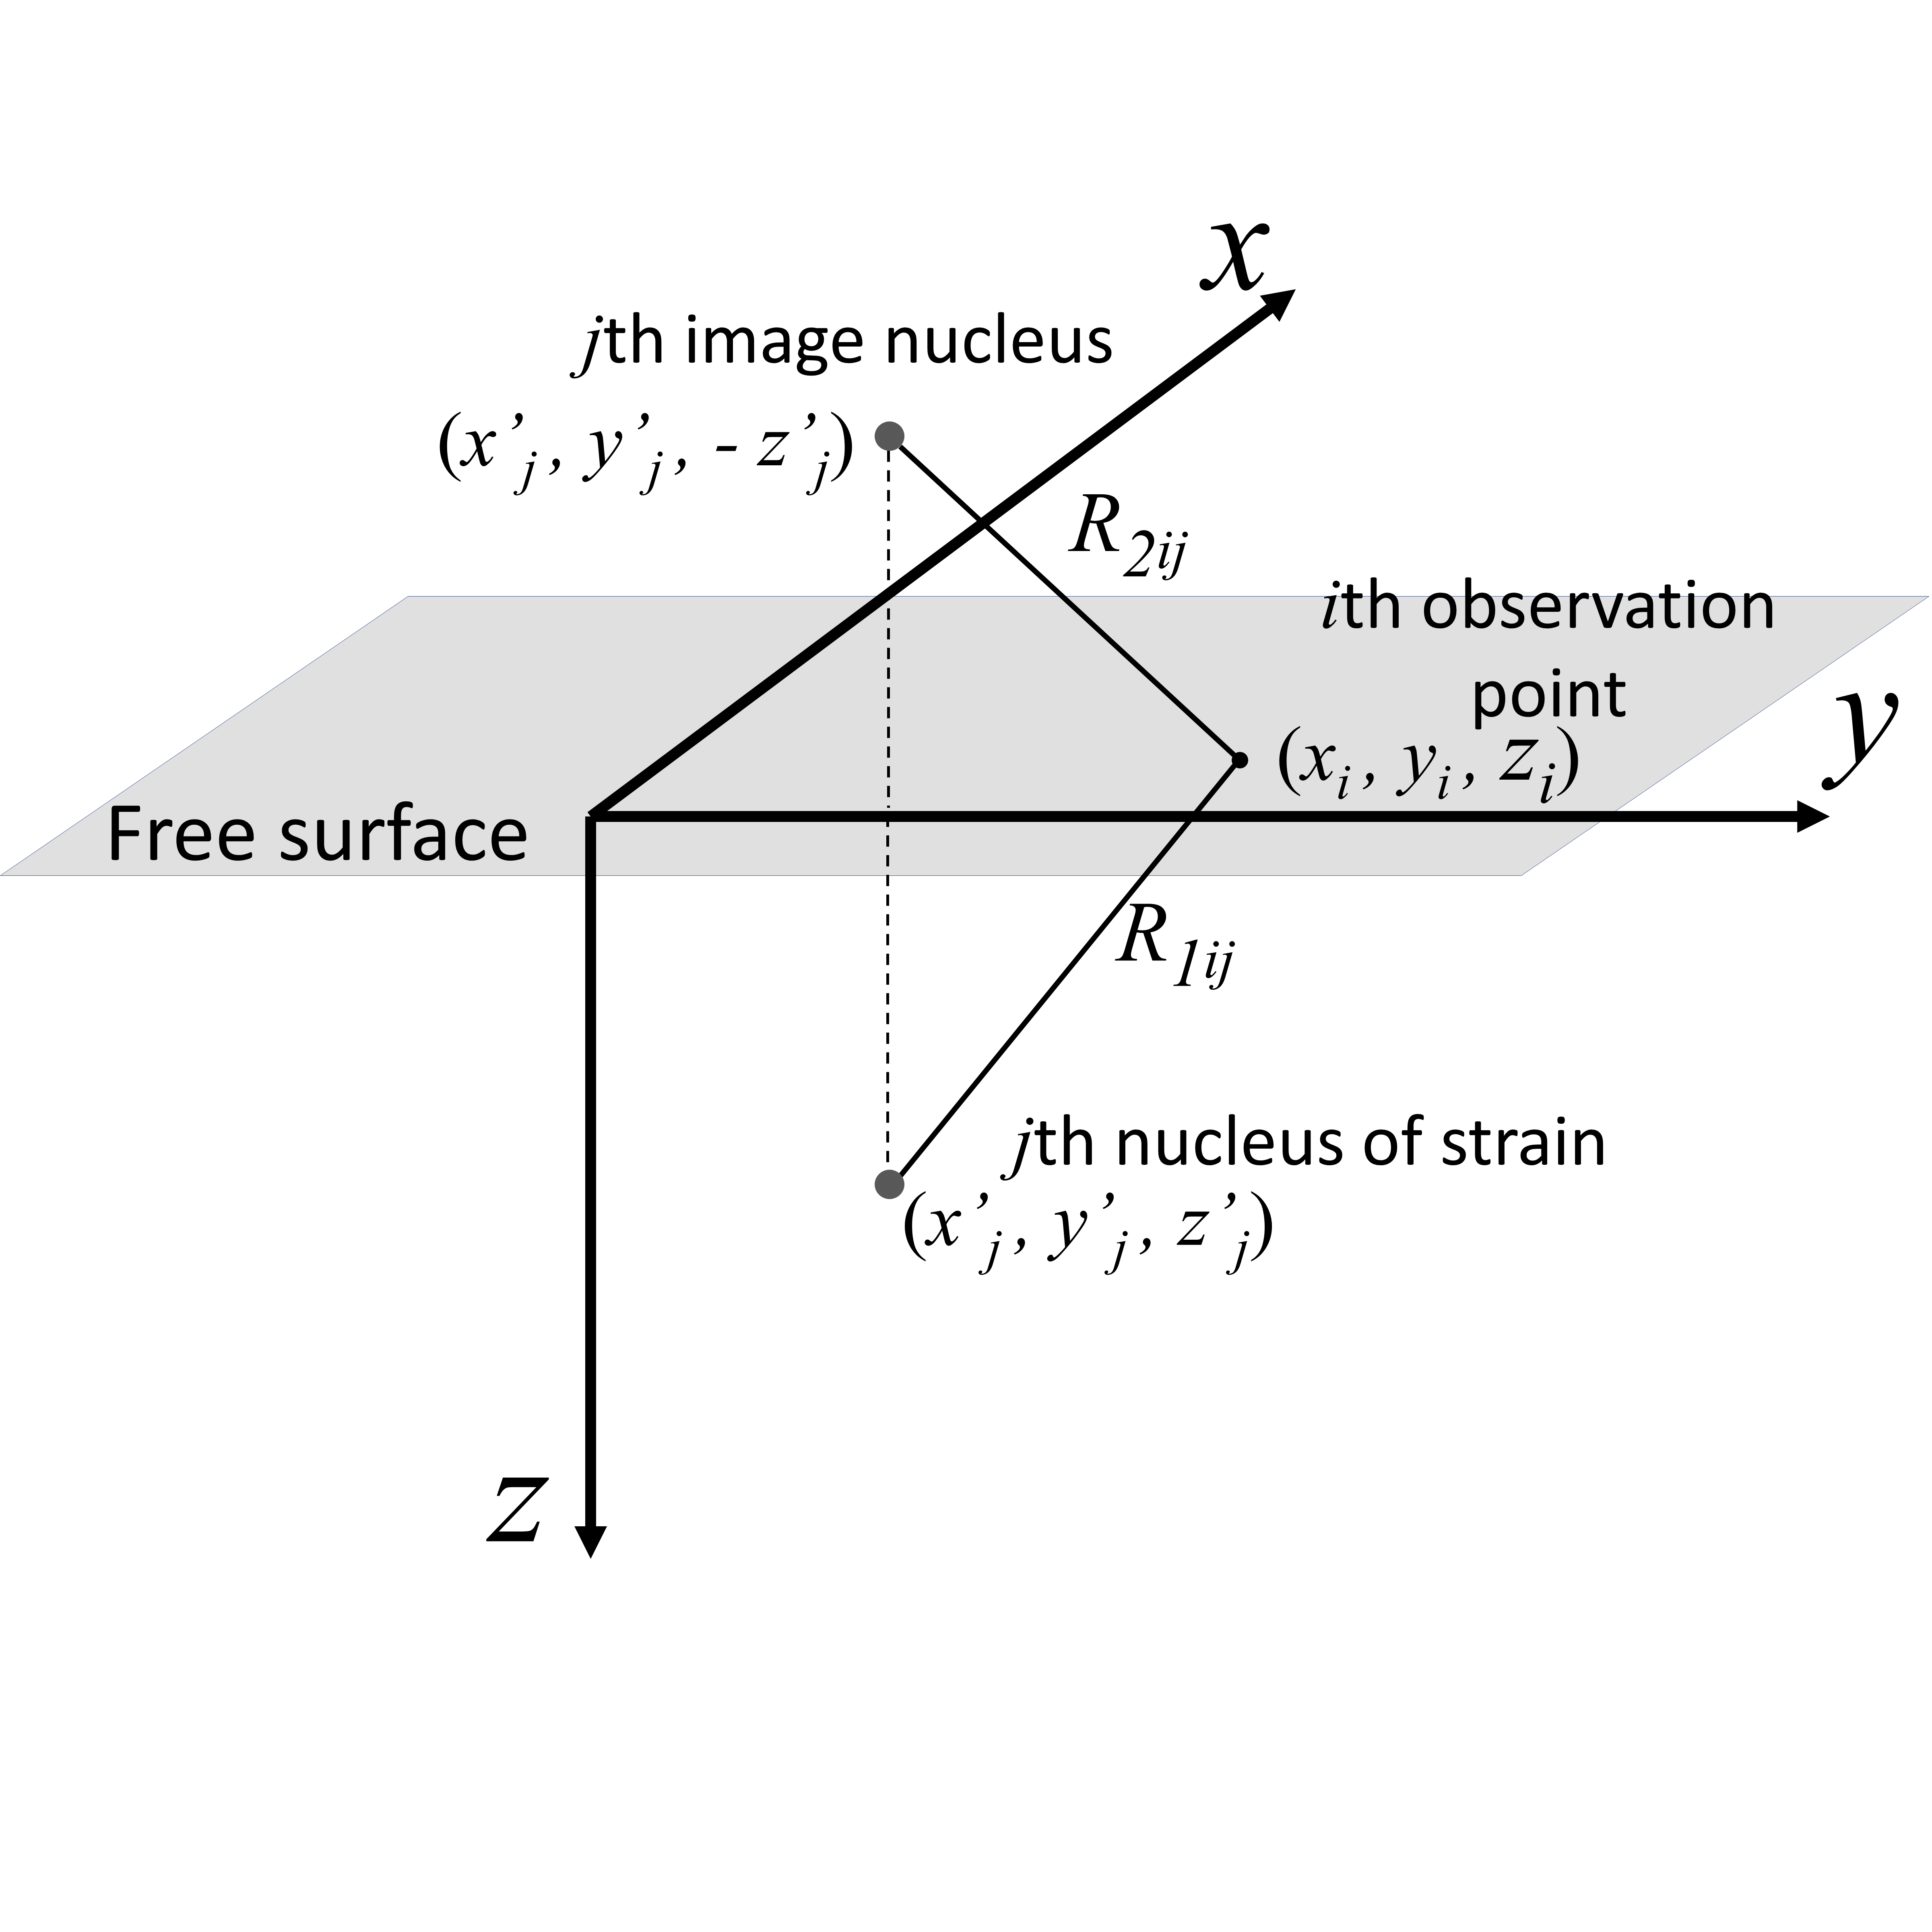
\includegraphics[scale=0.90]{figures/Figure_Nucleus_Strain.png}
    \vspace{-2.5cm} 
    \caption{Schematic representation of the geometry of the nucleus of strain in a semi-infinite medium. 
    After \cite{Munoz-Roehl17}. 
	The adopted Cartesian coordinate system considered the $x-$axis pointing to north, the $y-$axis pointing 
	to east and the $z-$axis pointing downward.}
	\label{fig:nucleus_strain}
\end{figure}

\noindent{\textbf{The discrete displacement forward modeling due to a reservoir in a homogeneous elastic semi-infinite medium}} 
%======================================================================================
%\subsection*{The discrete displacement forward modeling due to a %reservoir in a homogeneous elastic semi-infinite medium} \label{u-%model}
%======================================================================================

We parameterize the reservoir as a grid of juxtaposed right rectangular prisms.
Each grid prism undergoes a constant pressure change $\Delta p_{j}$; however, $\Delta p_{j}$
can be different for every prism. 
To calculate the displacement field produced by the $j$th prism
at the $i$th coordinates  $(x_i, y_i, z_i)$, we integrate the solution deduced for a single nucleus of strain (equation \ref{eq:displacement_ui})
over its volume and obtain
%\vspace{-1cm}
\begin{equation}
{\bf{\tilde{u}}}_{ij} = 
\iiint\limits_{{v_{1}}_{j}}
{\bf{u_{1}}}_{ij} dv_{j}^{\prime}
 + 
\iiint\limits_{{v_{2}}_{j}}
{\bf{u_{2}}}_{ij} \:\:  dv_{j}^{\prime},
\label{eq:nucleus-ui_jth_prism}
\end{equation}
where both integrals are conducted with respect to the variables 
$(x^{\prime}_{j}, y^{\prime}_{j}, z^{\prime}_{j})$. The first integral in equation 
\ref{eq:nucleus-ui_jth_prism} is conducted over the volume ${v_{1}}_{j}$ of the $j$th
prism and the second is conducted over the volume 
${v_{2}}_{j}$ of a different prism symmetrically positioned above the free surface 
and conveniently called $j$th "image prism".
Volume ${v_{1}}_{j}$ is defined by ${x_1}_{j}$, ${x_2}_{j}$, ${y_1}_{j}$, ${y_2}_{j}$,
${z_1}_{j}$, and ${z_2}_{j}$, which represent, respectively, the south, north, west, 
east, top, and bottom borders of the $j$th prism.
Volume ${v_{2}}_{j}$ of the $j$th image prism is defined in a similar way, but with 
top and bottom given by ${z_1}_{j} - 2 \, {z_c}_{j}$ and ${z_2}_{j} - 2 \, {z_c}_{j}$, where 
${z_c}_{j} = \frac{1}{2}({z_1}_{j} + {z_2}_{j})$ is the center depth of the $j$th prism.
The total displacement vector at the point $(x_i, y_i, z_i)$ due to the
pressure change in the whole reservoir is defined as the sum of the displacements 
${\bf{u}}_{ij}$ (equation \ref{eq:nucleus-ui_jth_prism}) yielded by each prism 
with constant pressure $\Delta p_{j}$:
%\vspace{-0.5cm}
\begin{equation}
{\bf{\tilde{u}}}_{i} = \sum_{j=1}^{M} {\bf{\tilde{u}}}_{ij},
\label{eq:nucleus-ui_M_prisms}
\end{equation}
where $M$ is the number of prisms setting up the reservoir model.
The horizontal component of the total displacement vector ${\bf{\tilde{u}}}_{i}$ 
(equation \ref{eq:nucleus-ui_M_prisms}) is calculated by 
%\vspace{-1cm}
\begin{equation}
{\tilde{u}}_{{i}_h} = \sqrt{ {\tilde{u}}_{{i}_x}^{2}  +  {\tilde{u}}_{{i}_y}^{2} },
\label{eq:horizontal_displacement}
\end{equation}
where ${\tilde{u}}_{{i}_x}$ and ${\tilde{u}}_{{i}_y}$ are the $x-$ and $y-$ components.
By substituting equations \ref{eq:nucleus-u1-vector} and \ref{eq:nucleus-u2-vector} 
into equation \ref{eq:nucleus-ui_jth_prism}, we obtain
%\vspace{-1cm}
\begin{equation}
\begin{aligned}
{\tilde{u}}_{{ij}_\alpha} = 
 A_{E} 
 &  \Delta p_{j}  
 \bigg[ \iiint\limits_{{v_{1}}_{j}} 
\frac{\partial }{\partial \alpha} {\frac{1}{{R_1}_{ij}}}  dv_{j}^{\prime} \: + \\ 
& C_{\nu} \: \iiint\limits_{{v_{2}}_{j}}
\frac{\partial }{\partial \alpha} {\frac{1}{{R_2}_{ij}}}  dv_j \: + \\ 
& 2  z_{i}  \iiint\limits_{{v_{2}}_{j}}
\frac{\partial^{2}  }{\partial \alpha \partial z} {\frac{1}{{R_2}_{ij}}} dv_{j}^{\prime} \bigg], 
\end{aligned}
\label{eq:u_til_alpha}
\end{equation}
where $\alpha = x, y$, and
%\vspace{-1cm}
\begin{equation}
\begin{aligned}
{\tilde{u}}_{{ij}_z} = 
A_{E} 
& \Delta p_{j}  \bigg[ \iiint\limits_{{v_{1}}_{j}}
\frac{\partial }{\partial z} {\frac{1}{{R_1}_{ij}}} dv_{j}^{\prime} \: - \\
& C_{\nu}  \: \iiint\limits_{{v_{2}}_{j}}
\frac{\partial }{\partial z} {\frac{1}{{R_2}_{ij}}} dv_{j}^{\prime} \: + \\ 
& 2 z_{i}  \iiint\limits_{{v_{2}}_{j}}
\frac{\partial^{2}  }{\partial z^{2}} {\frac{1}{{R_2}_{ij}}}  dv_{j}^{\prime} \bigg] .
\end{aligned}
\label{eq:u_til_z}
\end{equation}
In the right-hand side of equations \ref{eq:u_til_alpha} and \ref{eq:u_til_z}, the three integrals have the same form of derivatives of the gravitational potential produced by the $j$th prism and image prism. 
The first integral corresponds to the $\alpha-$component of the gravitational attraction 
produced by the $j$th prism.
The second and third integrals correspond, respectively, to the $\alpha-$component of the gravitational attraction and to the $\alpha \:z-$component of the gravitational 
gradient tensor produced by the $j$th image prism. 
The similarity between the displacement fields due to a volume source in a half-space and the gravitational field allows the use of closed expressions of the gravitational potential and its derivatives produced by the 3D right rectangular prism.  
We draw the readers' attention to the fact that \cite{Vasco1987} were the pioneer in taking the advantage of the similarity between the the displacement fields due to a source in a half-space and the gravitational field and calculating displacement field due to a 2D volume source at the Earth surface.
Here, our approach also takes the advantage of this similarity, but it calculates the displacement field due to a 3D volume source at the whole subsurface. 
In equations  \ref{eq:u_til_alpha} and \ref{eq:u_til_z}, the integrals depending on 
first derivatives of ${\frac{1}{{R_1}_{ij}}}$ have the following closed solutions 
\citep{Nagyetal2000, Nagyetal2002}:
%\vspace{-0.5cm}
\begin{equation}
\int\limits_{{x_{1}}_{j}}^{{x_{2}}_{j}} \int\limits_{{y_{1}}_{j}}^{{y_{2}}_{j}} \int\limits_{{z_{1}}_{j}}^{{z_{2}}_{j}}
\frac{\partial }{\partial x} {\frac{1}{{R_1}_{ij}}} dv_{j}^{\prime} \! = \!
\Bigg|\Bigg|\Bigg| 
y L_z  + z L_y -  x  T_{yz} 
\Bigg|_{{X_1}_{j}}^{{X_2}_{j}} \Bigg|_{{Y_1}_{j}}^{{Y_2}_{j}} \Bigg|_{{Z_1}_{j}}^{{Z_2}_{j}} \quad ,
\label{dx1}
\end{equation}
\vspace{-0.5cm}
\begin{equation}
\int\limits_{{x_{1}}_{j}}^{{x_{2}}_{j}} \int\limits_{{y_{1}}_{j}}^{{y_{2}}_{j}} \int\limits_{{z_{1}}_{j}}^{{z_{2}}_{j}}
\frac{\partial }{\partial y} {\frac{1}{{R_1}_{ij}}} dv_{j}^{\prime} \! = \!
\Bigg|\Bigg|\Bigg|
x L_z + z L_x -  y  T_{xz} 
\Bigg|_{{X_1}_{j}}^{{X_2}_{j}} \Bigg|_{{Y_1}_{j}}^{{Y_2}_{j}} \Bigg|_{{Z_1}_{j}}^{{Z_2}_{j}} \quad ,
\label{dy1}
\end{equation}
and
%\vspace{-0.5cm}
\begin{equation}
\int\limits_{{x_{1}}_{j}}^{{x_{2}}_{j}} \int\limits_{{y_{1}}_{j}}^{{y_{2}}_{j}} \int\limits_{{z_{1}}_{j}}^{{z_{2}}_{j}}
\frac{\partial }{\partial z} {\frac{1}{{R_1}_{ij}}} dv_{j}^{\prime} \! = \!
\Bigg|\Bigg|\Bigg|
x L_y  + y L_x  -  z  T_{xy} 
\Bigg|_{{X_1}_{j}}^{{X_2}_{j}} \Bigg|_{{Y_1}_{j}}^{{Y_2}_{j}} \Bigg|_{{Z_1}_{j}}^{{Z_2}_{j}} \quad ,
\label{dz1}
\end{equation}
where all derivatives are computed with respect to the coordinates of the $i$th point 
$(x_i, y_i, z_i)$, and $L_x = \ln(x + R), L_y = \ln(y + R) \textrm{and} L_z = \ln(z + R)$,
$T_{yz} = \tan^{-1} \big( \frac{yz}{x \: R} \big), T_{xz}  = \tan^{-1} \big( \frac{xz}{y \: R} \big)$  
and $T_{xy} = \tan^{-1} \big( \frac{xy}{z \: R} \big)$,  
$R = \sqrt{x^{2} + y^{2} + z^{2}}$. 
The integration limits in equations \ref{dx1}--`\ref{dz1} are
%\vspace{-1cm}
%\begin{equation}
%{X_1}_{j} = x_i - {x_1}_{j}, \:
%{X_2}_{j} = x_i - {x_2}_{j}, \:
%{Y_1}_{j} = y_i - {y_1}_{j}, \:
%{Y_2}_{j} = y_i - {y_2}_{j}, \:
%{Z_1}_{j} = z_i - {z_1}_{j}, \: \textrm{and} \:
%{Z_2}_{j} = z_i - {z_2}_{j}.
%\label{eq:Nagy_limits_1}
%\end{equation}
\begin{equation}
\begin{array}{ll}
{X_1}_{j} &= x_i - {x_1}_{j} , \\
{X_2}_{j} &= x_i - {x_2}_{j} , \\
{Y_1}_{j} &= y_i - {y_1}_{j} , \\
{Y_2}_{j} &= y_i - {y_2}_{j} , \\
{Z_1}_{j} &= z_i - {z_1}_{j} , \: \: \: \textrm{and}  \\
{Z_2}_{j} &= z_i - {z_2}_{j}.
\end{array} \quad
\label{eq:Nagy_limits_1}
\end{equation}
The remaining integrals, in the right-hand side of equations 
\ref{eq:u_til_alpha} and \ref{eq:u_til_z}, depend on first and second derivatives 
of ${\frac{1}{{R_2}_{ij}}}$.
These integrals are conducted over the volume ${v_{2}}_{j}$ of the $j$th image prism and have the following closed solutions \citep{Nagyetal2000, Nagyetal2002}:
%\vspace{-0.5cm}
\begin{equation}
\int\limits_{{x_{1}}_{j}}^{{x_{2}}_{j}} \! 
\int\limits_{{y_{1}}_{j}}^{{y_{2}}_{j}} \! 
\int\limits_{{z_{1}}_{j} - 2 \,  z_c}^{{z_{2}}_{j} - 2 \, z_c} 
\! \! \! \! \! \! \! 
\frac{\partial}{\partial x} \! {\frac{1}{{R_2}_{ij}}} dv_{j}^{\prime} \! = \!
\Bigg|\Bigg|\Bigg| 
y L_z  + z L_y  -  x  T_{yz}  \!
\Bigg|_{{X_1}_{j}}^{{X_2}_{j}} \! \Bigg|_{{Y_1}_{j}}^{{Y_2}_{j}} \! \Bigg|_{{Z_1}_{j}}^{{Z_2}_{j}},
\label{dx2}
\end{equation}
\vspace{-0.5cm}
\begin{equation}
\int\limits_{{x_{1}}_{j}}^{{x_{2}}_{j}} \! 
\int\limits_{{y_{1}}_{j}}^{{y_{2}}_{j}} 
\int\limits_{{z_{1}}_{j} - 2 \, z_c}^{{z_{2}}_{j} - 2 \, z_c}
\! \! \! \! \! \! \! \!  
\frac{\partial}{\partial y} {\frac{1}{{R_2}_{ij}}} dv_{j}^{\prime} \! = \!
\Bigg|\Bigg|\Bigg|
xL_z + zL_x -  y T_{xz} \!
\Bigg|_{{X_1}_{j}}^{{X_2}_{j}} \! \Bigg|_{{Y_1}_{j}}^{{Y_2}_{j}} \! \Bigg|_{{Z_1}_{j}}^{{Z_2}_{j}},
\label{dy2}
\end{equation}
\vspace{-0.5cm}
\begin{equation}
\int\limits_{{x_{1}}_{j}}^{{x_{2}}_{j}} \! 
\int\limits_{{y_{1}}_{j}}^{{y_{2}}_{j}} 
\int\limits_{{z_{1}}_{j} - 2 \, z_c}^{{z_{2}}_{j} - 2 \, z_c}
\! \! \! \! \! \! \! \! 
\frac{\partial }{\partial z} {\frac{1}{{R_2}_{ij}}} dv_{j}^{\prime} \! = \!
\Bigg|\Bigg|\Bigg|
x L_y  + y L_x -  z T_{xy} \!
\Bigg|_{{X_1}_{j}}^{{X_2}_{j}} \! \Bigg|_{{Y_1}_{j}}^{{Y_2}_{j}} \! \Bigg|_{{Z_1}_{j}}^{{Z_2}_{j}} ,
\label{dz2}
\end{equation}
\vspace{-0.5cm}
\begin{equation}
\int\limits_{{x_{1}}_{j}}^{{x_{2}}_{j}} \!
\int\limits_{{y_{1}}_{j}}^{{y_{2}}_{j}} 
\int\limits_{{z_{1}}_{j} - 2 \, z_c}^{{z_{2}}_{j} - 2 \, z_c}
\! \! \! \! \! \! \! \! 
\frac{\partial^{2}}{\partial x \partial z} {\frac{1}{{R_2}_{ij}}} dv_{j}^{\prime} \! = \!
\Bigg|\Bigg|\Bigg| 
L_y \!
\Bigg|_{{X_1}_{j}}^{{X_2}_{j}} \! \Bigg|_{{Y_1}_{j}}^{{Y_2}_{j}} \! \Bigg|_{{Z_1}_{j}}^{{Z_2}_{j}} ,
\label{dxz2}
\end{equation}
%\vspace{-0.5cm}
\begin{equation}
\int\limits_{{x_{1}}_{j}}^{{x_{2}}_{j}} \!
\int\limits_{{y_{1}}_{j}}^{{y_{2}}_{j}} 
\int\limits_{{z_{1}}_{j} - 2 \, z_c}^{{z_{2}}_{j} - 2 \, z_c}
\! \! \! \! \! \! \! \! 
\frac{\partial^{2}}{\partial y \partial z} {\frac{1}{{R_2}_{ij}}} dv_{j}^{\prime} \! = \!
\Bigg|\Bigg|\Bigg|
L_x \!
\Bigg|_{{X_1}_{j}}^{{X_2}_{j}} \! \Bigg|_{{Y_1}_{j}}^{{Y_2}_{j}} \! \Bigg|_{{Z_1}_{j}}^{{Z_2}_{j}} ,
\label{dyz2}
\end{equation}
and
%\vspace{-0.5cm}
\begin{equation}
\int\limits_{{x_{1}}_{j}}^{{x_{2}}_{j}} \!
\int\limits_{{y_{1}}_{j}}^{{y_{2}}_{j}} 
\int\limits_{{z_{1}}_{j} - 2 \, z_c}^{{z_{2}}_{j} - 2 \, z_c}
\! \! \! \! \! \! \! \! 
\frac{\partial^{2}}{\partial z \partial z} {\frac{1}{{R_2}_{ij}}} dv_{j}^{\prime} \! = \!
\Bigg|\Bigg|\Bigg|
-  T_{xy} 
\Bigg|_{{X_1}_{j}}^{{X_2}_{j}} \! \Bigg|_{{Y_1}_{j}}^{{Y_2}_{j}} \!  \Bigg|_{{Z_1}_{j}}^{{Z_2}_{j}} \quad .
\label{dzz2}
\end{equation}
In these integrals related to the $j$th image prism 
(equations \ref{dx2}--\ref{dz2}), the integration limits along the $z$ direction
are given by
%\vspace{-1cm}
\begin{equation}
{Z_1}_{j} = z_i - {z_1}_{j} + 2 \, {z_c}_{j} \:\: \: \textrm{and} \: \: \:
{Z_2}_{j} = z_i - {z_2}_{j} + 2 \, {z_c}_{j} \:,
\label{eq:Nagy_limits_2}
\end{equation}
%\begin{equation}
%\begin{array}{ll}
%{Z_1}_{j} &= z_i - {z_1}_{j} + 2 \, {z_c}_{j} \\
%{Z_2}_{j} &= z_i - {z_2}_{j} + 2 \, {z_c}_{j}
%\end{array} \quad ,
%\label{eq:Nagy_limits_2}
%\end{equation}
where ${z_c}_{j} = \frac{1}{2}({z_1}_{j} + {z_2}_{j})$ is the center depth of the $j$th prism. 
The remaining limits along $x$ and $y$ directions are the same defined by equation \ref{eq:Nagy_limits_1}.

\vspace{0.5cm}
\noindent{\textbf{The discrete stress forward modeling due to a reservoir in a homogeneous elastic semi-infinite medium}}
%======================================================================================
%\subsection*{The discrete stress forward modeling due to a reservoir %in a homogeneous elastic semi-infinite medium}
%======================================================================================

By following the similar approach used in the previous subsection, the stress field of each prism assuming constant pressure is calculated by integrating solution for a 
nucleus of strain (equations \ref{eq:stress_nucleus}, \ref{eq:nucleus-stress1-vector},
and \ref{eq:nucleus-stress2-vector}) over its volume. 
This integration leads to a stress vector 
$\mbox{\boldmath$\tilde{\sigma}$}_{ij} \equiv \mbox{\boldmath$\tilde{\sigma}$}(x_{i}, y_{i}, z_{i}, x^{\prime}_{j}, y^{\prime}_{j}, z^{\prime}_{j})$ given by
%\vspace{-1cm}
\begin{equation}
\mbox{\boldmath$\tilde{\sigma}$}_{ij} = 
\iiint\limits_{{v_{1}}_{j}}
\mbox{\boldmath$\sigma_{1}$}_{ij} dv_{j}^{\prime}
+ 
\iiint\limits_{{v_{2}}_{j}}
\mbox{\boldmath$\sigma_{2}$}_{ij} dv_{j}^{\prime},
\label{eq:nucleus-stress_jth_prism}
\end{equation}
where the first and second integrals are conducted, respectively, over the volumes 
${v_{1}}_{j}$ and ${v_{2}}_{j}$ of the $j$th prism and the $j$th image prism.
The total stress vector at the $i$th coordinates  $(x_i, y_i, z_i)$ due to the pressure change in the whole reservoir is calculated by the sum of all stress vector $\mbox{\boldmath$\tilde{\sigma}$}_{ij}$ (equation \ref{eq:nucleus-stress_jth_prism}), i.e., 
%\vspace{-1cm}
\begin{equation}
\mbox{\boldmath$\tilde{\sigma}$}_{i} = 
\sum_{j=1}^{M} \mbox{\boldmath$\tilde{\sigma}$}_{ij} \: .
\label{eq:nucleus-stress_M_prisms}
\end{equation}
By substituting equation \ref{eq:nucleus-stress1-vector} and 
\ref{eq:nucleus-stress2-vector} into equation \ref{eq:nucleus-stress_jth_prism}, 
we obtain the $\alpha-$component (where  $\alpha = x$ and $y$) and the $z-$ component 
of the stress vector $\mbox{\boldmath$\tilde{\sigma}$}_{ij}$ as follows:
%\vspace{-0.5cm}
\begin{equation}
\begin{aligned}
{\tilde{\sigma}}_{{ij}_\alpha} \! = \! A  
& \Delta p_{j} \! \Bigg[
\iiint\limits_{{v_{1}}_{j}} \!\!
\frac{\partial^{2}}{\partial \alpha \partial z} {\frac{1}{{R_1}_{ij}}}  dv_{j}^{\prime}
\! +  \!  \iiint\limits_{{v_{2}}_{j}}
\frac{\partial^{2} }{\partial \alpha \partial z} {\frac{1}{{R_2}_{ij}}} dv_{j}^{\prime} \\
& +  2  z_{i} \iiint\limits_{{v_{2}}_{j}}
\frac{\partial^{3}}{\partial \alpha \partial z ^{2}} {\frac{1}{{R_2}_{ij}}}  dv_{j}^{\prime} \Bigg]
\end{aligned}
\label{eq:stress_til_alpha}
\end{equation}
and 
%\vspace{-0.5cm}
\begin{equation}
\begin{aligned}
{\tilde{\sigma}}_{{ij}_{z}} \! = \! A  
& \Delta p_{j} \!  \Bigg[
\iiint\limits_{{v_{1}}_{j}} \! \! 
\frac{\partial^{2}}{\partial z^{2}} {\frac{1}{{R_1}_{ij}}}  dv_{j}^{\prime}
\! + \!\iiint\limits_{{v_{2}}_{j}}
\frac{\partial^{2} }{\partial z^{2}} {\frac{1}{{R_2}_{ij}}} dv_{j}^{\prime} \\
& + 2 z_{i}  \iiint\limits_{{v_{2}}_{j}}
\frac{\partial^{3}  }{\partial z^{3}} {\frac{1}{{R_2}_{ij}}}  
dv_{j}^{\prime} \Bigg].
\end{aligned}
\label{eq:stress_til_z}
\end{equation}
Similarly to the displacement field (equations \ref{eq:u_til_alpha} and \ref{eq:u_til_z}), the three integrals in the right-hand side of equations \ref{eq:stress_til_alpha} and \ref{eq:stress_til_z} have the same form of 
derivatives of the gravitational potential produced by the $j$th prism and image prism.
The integrals depending on $\frac{1}{{R_1}_{ij}}$ have the following closed 
solutions \citep{Nagyetal2000, Nagyetal2002}:
%\vspace{-0.5cm}
\begin{equation}
\int\limits_{{x_{1}}_{j}}^{{x_{2}}_{j}} \int\limits_{{y_{1}}_{j}}^{{y_{2}}_{j}} \int\limits_{{z_{1}}_{j}}^{{z_{2}}_{j}} 
\! \! \!
\frac{\partial^{2}  }{\partial x \partial z}{\frac{1}{{R_1}_{ij}}} dv_{j}^{\prime} = 
\Bigg|\Bigg|\Bigg| L_y 
\Bigg|_{{X_1}_{j}}^{{X_2}_{j}} \Bigg|_{{Y_1}_{j}}^{{Y_2}_{j}} \Bigg|_{{Z_1}_{j}}^{{Z_2}_{j}} \quad ,
\label{dxz1}
\end{equation}
%\vspace{-0.5cm}
\begin{equation}
\int\limits_{{x_{1}}_{j}}^{{x_{2}}_{j}} \int\limits_{{y_{1}}_{j}}^{{y_{2}}_{j}} \int\limits_{{z_{1}}_{j}}^{{z_{2}}_{j}}
\! \! \!
\frac{\partial^{2}  }{\partial y \partial z} {\frac{1}{{R_1}_{ij}}} dv_{j}^{\prime} =
\Bigg|\Bigg|\Bigg|
L_x
\Bigg|_{{X_1}_{j}}^{{X_2}_{j}} \Bigg|_{{Y_1}_{j}}^{{Y_2}_{j}} \Bigg|_{{Z_1}_{j}}^{{Z_2}_{j}} \quad ,
\label{dyz1}
\end{equation}
and
%\vspace{-0.5cm}
\begin{equation}
\int\limits_{{x_{1}}_{j}}^{{x_{2}}_{j}} \int\limits_{{y_{1}}_{j}}^{{y_{2}}_{j}} \int\limits_{{z_{1}}_{j}}^{{z_{2}}_{j}}
\! \! \!
\frac{\partial^{2}  }{\partial z \partial z} {\frac{1}{{R_1}_{ij}}} dv_{j}^{\prime} =
\Bigg|\Bigg|\Bigg|
-  T_{xy} \Bigg)
\Bigg|_{{X_1}_{j}}^{{X_2}_{j}} \Bigg|_{{Y_1}_{j}}^{{Y_2}_{j}} \Bigg|_{{Z_1}_{j}}^{{Z_2}_{j}} \quad ,
\label{dzz1}
\end{equation}
where the limits ${X_1}_{j}$, ${X_2}_{j}$, ${Y_1}_{j}$, ${Y_2}_{j}$, ${Z_1}_{j}$, and ${Z_2}_{j}$ are defined by equation \ref{eq:Nagy_limits_1}.
The integrals depending on second derivatives of $\frac{1}{{R_2}_{ij}}$ in the 
right-hand side of equations \ref{eq:stress_til_alpha} and \ref{eq:stress_til_z} 
have closed solutions defined by equations \ref{dxz2}, \ref{dyz2}, and \ref{dzz2}.
Finally, the remaining integrals depending on third derivatives of 
$\frac{1}{{R_2}_{ij}}$ have closed solutions given by 
\citep{Nagyetal2000, Nagyetal2002}:
%\vspace{-0.5cm}
\begin{equation}
\begin{aligned}
\int\limits_{{x_{1}}_{j}}^{{x_{2}}_{j}} 
\int\limits_{{y_{1}}_{j}}^{{y_{2}}_{j}} 
\int\limits_{{z_{1}}_{j} - 2 \, z_c}^{{z_{2}}_{j} - 2 \, z_c}
\! \! \! \! \! \! \! \! 
& \frac{\partial^{3}}{\partial x \partial z^{2}} 
{\frac{1}{{R_2}_{ij}}} dv_{j}^{\prime} \! = \! \\
& \Bigg|\Bigg|\Bigg| 
\frac{- y z}{R} 
\left( \frac{1}{x^{2} + z^{2}} \right)
\Bigg|_{{X_1}_{j}}^{{X_2}_{j}} \Bigg|_{{Y_1}_{j}}^{{Y_2}_{j}} \Bigg|_{{Z_1}_{j}}^{{Z_2}_{j}} \quad ,
\end{aligned}
\label{sxzz}
\end{equation}
%\vspace{-0.5cm}
\begin{equation}
\begin{aligned}
\int\limits_{{x_{1}}_{j}}^{{x_{2}}_{j}} \int\limits_{{y_{1}}_{j}}^{{y_{2}}_{j}} 
\int\limits_{{z_{1}}_{j} - 2 \, z_c}^{{z_{2}}_{j} - 2 \, z_c}
\! \! \! \! \! \! \! \! 
& \frac{\partial^{2}  }{\partial y \partial z^{2}} 
{\frac{1}{{R_2}_{ij}}} dv_{j}^{\prime} \! = \! \\
& \Bigg|\Bigg|\Bigg|
\frac{- x z}{R} 
\left( \frac{1}{y^{2} + z^{2}} \right)
\Bigg|_{{X_1}_{j}}^{{X_2}_{j}} \Bigg|_{{Y_1}_{j}}^{{Y_2}_{j}} \Bigg|_{{Z_1}_{j}}^{{Z_2}_{j}} \quad ,
\end{aligned}
\label{syzz}
\end{equation}
and
%\vspace{-0.5cm}
\begin{equation}
\begin{aligned}
\int\limits_{{x_{1}}_{j}}^{{x_{2}}_{j}} \int\limits_{{y_{1}}_{j}}^{{y_{2}}_{j}} \int\limits_{{z_{1}}_{j} - 2 \, z_c}^{{z_{2}}_{j} - 2 \, z_c}
\! \! \! \! \! \! \! \! 
& \frac{\partial^{3}  }{\partial z^{3}} 
{\frac{1}{{R_2}_{ij}}} dv_{j}^{\prime} \! = \! \\
& \Bigg|\Bigg|\Bigg|
\frac{ x y}{R} 
\left( \frac{1}{x^{2} + z^{2}} + \frac{1}{y^{2} + z^{2}} \right)
\Bigg|_{{X_1}_{j}}^{{X_2}_{j}} \Bigg|_{{Y_1}_{j}}^{{Y_2}_{j}} \Bigg|_{{Z_1}_{j}}^{{Z_2}_{j}} \quad ,
\end{aligned}
\label{sz3}
\end{equation}
where the limits ${X_1}_{j}$, ${X_2}_{j}$, ${Y_1}_{j}$, and ${Y_2}_{j}$, are defined by equation \ref{eq:Nagy_limits_1} and ${Z_1}_{j}$, and ${Z_2}_{j}$ by equation \ref{eq:Nagy_limits_2}.
Our method was implemented in Python programming language and it is based on Harmonica \citep{Uieda2020}.
The horizontal and vertical displacements are calculated by using 
the volume integrations (equations \ref{eq:u_til_alpha} and \ref{eq:u_til_z}), whose solutions
are given by equations \ref{dx1}--\ref{dzz2}. 
The horizontal and vertical stresses are calculated by using the volume integrations (equations \ref{eq:stress_til_alpha} and \ref{eq:stress_til_z}),
whose solutions are given by equations \ref{dxz1}--\ref{sz3}. 
We used \cite{Fukushima2020} to overcome the zero division in evaluating the arguments of the arctangent function.
%\noindent{\textbf{Software implementation}}
%======================================================================================
%\subsection*{Software implementation}
%======================================================================================

%The method proposed here was implemented in Python programming language and it is based on Harmonica \citep{Uieda2020}.
%The horizontal and vertical displacements are calculated by using 
%the full volume integrations (equations \ref{eq:u_til_alpha} and \ref{eq:u_til_z}), whose 
%closed solutions are given by equations \ref{dx1}--\ref{dzz2}. 
%Moreover, the horizontal and vertical stresses are calculated by using 
%the full volume integrations (equations \ref{eq:stress_til_alpha} and \ref{eq:stress_til_z}),
%whose closed solutions are given by equations \ref{dxz1}--\ref{sz3}. 
%In equations \ref{dx1}--\ref{dz1}, \ref{dx2}--\ref{dzz2} and \ref{dxz1}--\ref{dzz1}, we adopted the modifications proposed by \cite{Fukushima2020}.
%To overcome the zero division in evaluating the arguments of the arctangent function, \cite{Fukushima2020} replaced  $\tan^{-1} \big( \frac{S}{T} \big)$ by 
%\begin{equation}
%arctan2(S,T) = \begin{cases}
	%\left\{ \begin{aligned}
%    atan (S/T) & \:\: \mbox{if} \: \:\:  T \neq 0 \\
%    \pi /2 & \:\: \mbox{if} \: \:\:  T = 0  \: \: \mbox{and} \: \:S > %0 \\
%    -\pi /2 & \:\: \mbox{if} \: \:\:  T = 0  \: \: \mbox{and} \: \:S %0 \\
%    0 & \:\: \mbox{if} \: \:\:  T = 0  \: \: \mbox{and} \: \:S = 0 \\
%    %\end{aligned} \right\}.
%    \end{cases}
%\label{eq:arctan2}  
%\end{equation}
%Additionally, if the argument of the logarithm is less than $10^{-10}%$, the logarithm is replaced by zero; otherwise the logarithm is  calculated regularly.
%\vspace{-0.5cm}
\section*{Numerical Applications}

\noindent{\textbf{Disk-shaped reservoir under uniform depletion}}
%\subsection*{Disk-shaped reservoir under uniform depletion}

Embedded in a semi-infinite homogenous medium, we simulated a vertical cylinder-like reservoir (not shown) with a radius of 500 m and whose horizontal coordinates of its center along the north-south and east-west directions are 0 m and 0 m, respectively.
The depths to the top and to the bottom of the simulated reservoir are 750 m and 850 m, respectively.
The reservoir is uniformly depleted by $\Delta p = -10$ MPa. 
The Young’s modulus is  3300 (in MPa), the Poisson's coefficient is 0.25, and
the uniaxial compaction coefficient $C_{m}$  (equation \ref{eq:Cm}) is 
$2.2525 \: 10^{-4}$ $\textrm{ MPa}^{-1}$.
%\begin{figure}
%    \centering
%    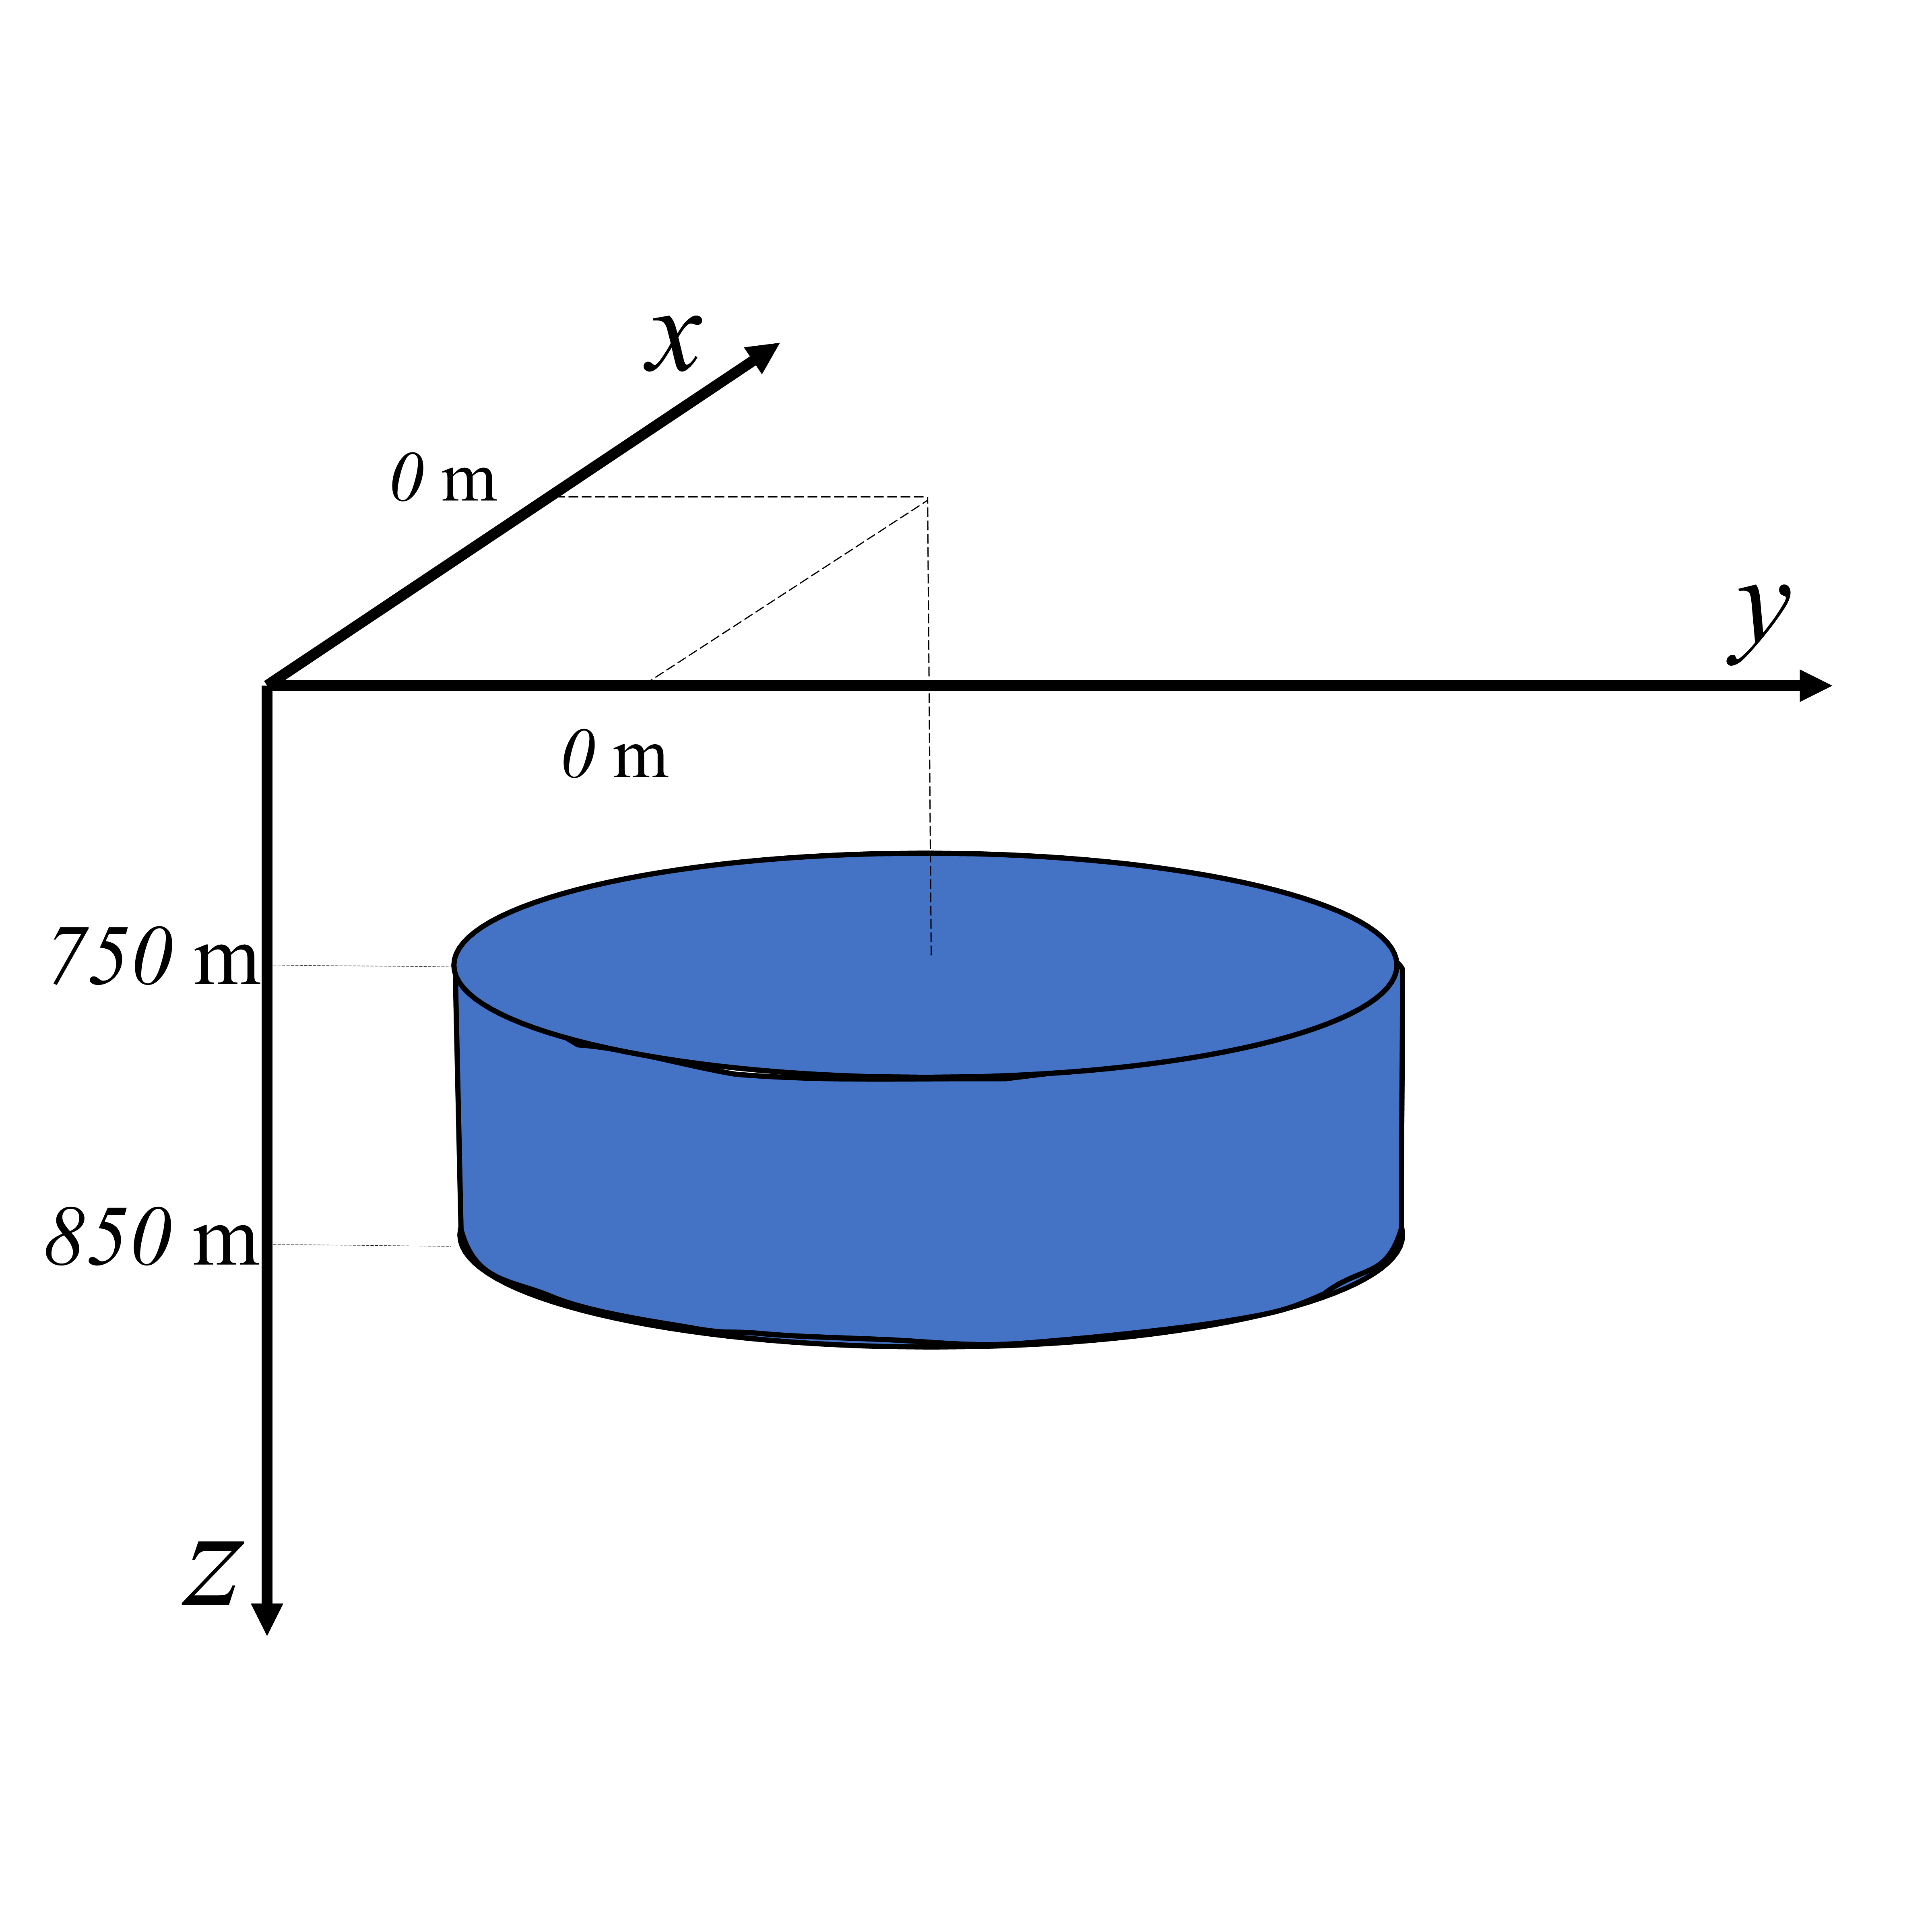
\includegraphics[scale=1.0]{figures/Figure_Cylinder.png}
%    \caption{Disk-shaped reservoir under uniform depletion with a radius of 500 m.}
%	\label{fig:cylinder}
%\end{figure}
To apply our methodology, we  discretized the cylinder  along the $x-$ and $y-$ directions into an $20 \times 20$ grid of prisms. Hence, we totalized 400 prisms all of them centered at 800 m deep, with depths to the top and to the bottom at 750 m and 850 m  and with pressure change $\Delta p_j$, $j = 1, ..., 400$ equal to $-10$ MPa.
To apply the Geertsma’s method \citep{Geertsma73}, we used the disk-shaped reservoir 
described in \cite{Fjaer08} with dimensions and physical properties defined above.
Figures \ref{fig:displacement}  and \ref{fig:displacement_Geertsma}  show cross-sections at 
$x  = 0$ m of the displacement fields in 2D contour plots  due to the pressure change in the whole  cylindrical reservoir by using our methodology and Geertsma’s method, respectively.
Because we defined the $z-$axis as positive downwards, the positive vertical displacement means a subsidence and the negative vertical displacement means an uplift.
Figure \ref{fig:displacement}  shows the horizontal and vertical displacements  calculated, respectively, with equations \ref{eq:horizontal_displacement} and \ref{eq:u_til_z} by our methodology.
Figure \ref{fig:displacement_Geertsma} shows the radial and vertical displacements using Geertsma’s method considering an elastic homogeneous cylindrical reservoir under uniform depletion based on the nucleus-of-strain concept in the half-space.
In both cases (Figures \ref{fig:displacement}b and \ref{fig:displacement_Geertsma}b) the vertical displacements due to the entire the disk-shaped reservoir display a subsidence (positive values) above the reservoir and an uplift (negative values) below the reservoir.
We stress that the proposed volume integrations  (equations \ref{dx1} $-$ \ref{dzz2})  allowed  to evaluate the  vertical displacement (Figure \ref{fig:displacement}b) throughout  the entire reservoir.
Rather, the  vertical displacement using Geertsma’s method 
(Figure \ref{fig:displacement_Geertsma}b) is only valid outside the reservoir. 
The radial displacement using Geertsma’s method 
(Figure \ref{fig:displacement_Geertsma}a) shows positive values at the edges of the reservoir ($y= -500$ and $y = 500$) with a singularity at the center of the reservoir 
($x= 0, \: y = 0$ and $z = 800$ m). 
The horizontal displacement with the proposed full integration 
(Figures \ref{fig:displacement}a) shows positive values at the edges of the reservoir ($y= -500$ and $y = 500$); however, it does not present sigularities inside the reservoir.
Figure \ref{fig:displacement_z_levels} shows the $x-$component displacement and vertical displacement by our methodology that uses a full volume integrations.
These displacements are calculated along the $x-$axis, at $y = 0$ m and considering four surfaces located at the following depths:  seafloor ($z = 0$ m), reservoir top ($z = 750$ m), reservoir center ($z = 800$ m) and reservoir bottom ($z = 850$ m).
In the $x$-component of the displacement (Figure \ref{fig:displacement_z_levels}a), we can note an increased horizontal contraction from the center of the reservoir ($x = 0$) toward the reservoir edge ($x= 500$ m) where the maximum contraction of all surfaces occur.
In the vertical displacement (Figure \ref{fig:displacement_z_levels}b), we can note a subsidence of the seafloor and the reservoir top (positive values) and an uplift of the reservoir bottom (negative values).
The vertical displacements of the seafloor, the top and bottom of the reservoir for Geertsma’s method (Figure \ref{fig:displacement_z_levels_Geertsma}) show a similar behavior of those obtained by our methodology that uses a full volume integrations (Figure \ref{fig:displacement_z_levels}b). 
However, we note that the subsidence of the seafloor is more attenuated in the Geertsma’s method than in our method because we calculate the total displacement field outside and inside of the reservoir.
This fact is important because the moviment of the seafloor should be monitored in hydrocarbon fields under production.
Figure \ref{fig:Null_stress} shows the null stress through the free surface at the plane $z=0$ m due to reservoir under uniform depletion.
\begin{figure}[h]
    \centering
    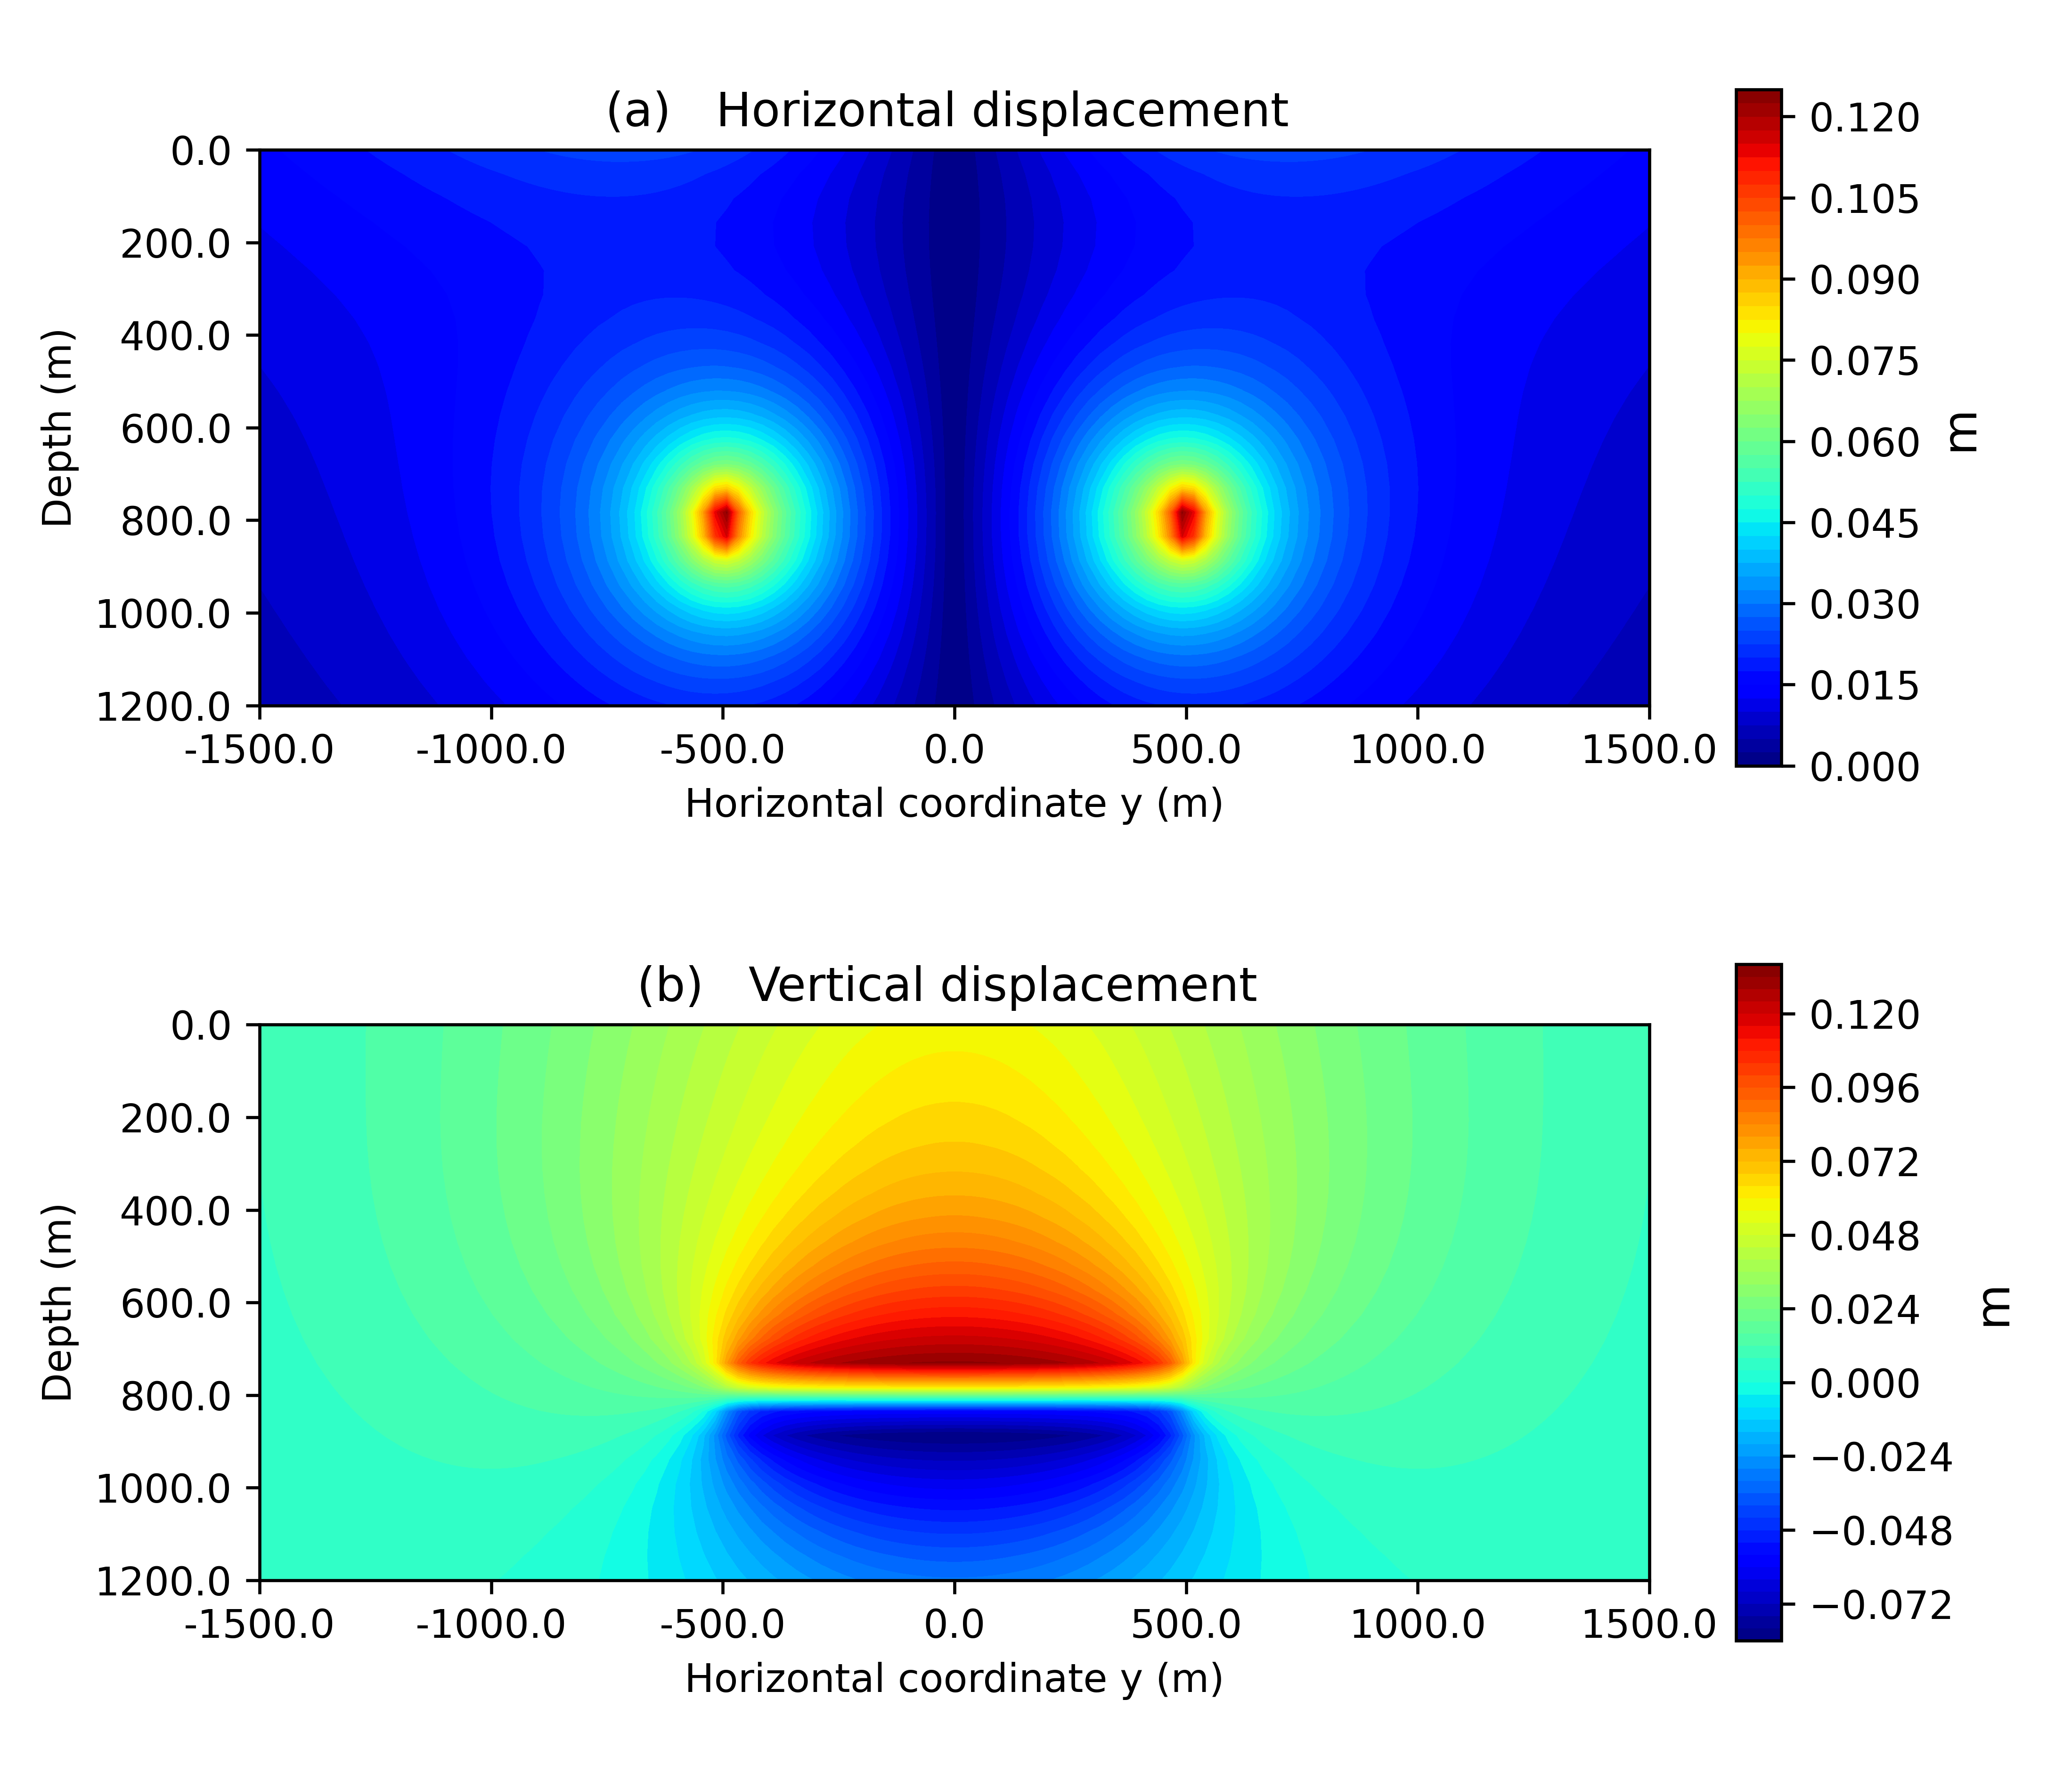
\includegraphics[scale=0.40]{figures/Figure_Displacement.png}
    \caption{Reservoir under uniform depletion: (a) horizontal displacement (equation 
	\ref{eq:horizontal_displacement}) and (b) vertical displacement (equation \ref{eq:u_til_z}) by our 
	methodology that uses the closed expressions of the volume integrations (equations \ref{eq:u_til_alpha} 
	and \ref{eq:u_til_z}), whose closed solutions are given by equations \ref{dx1}--\ref{dzz2}.}
	\label{fig:displacement}
\end{figure}
\vspace{0.00mm} 
\begin{figure}[h]
    \centering
    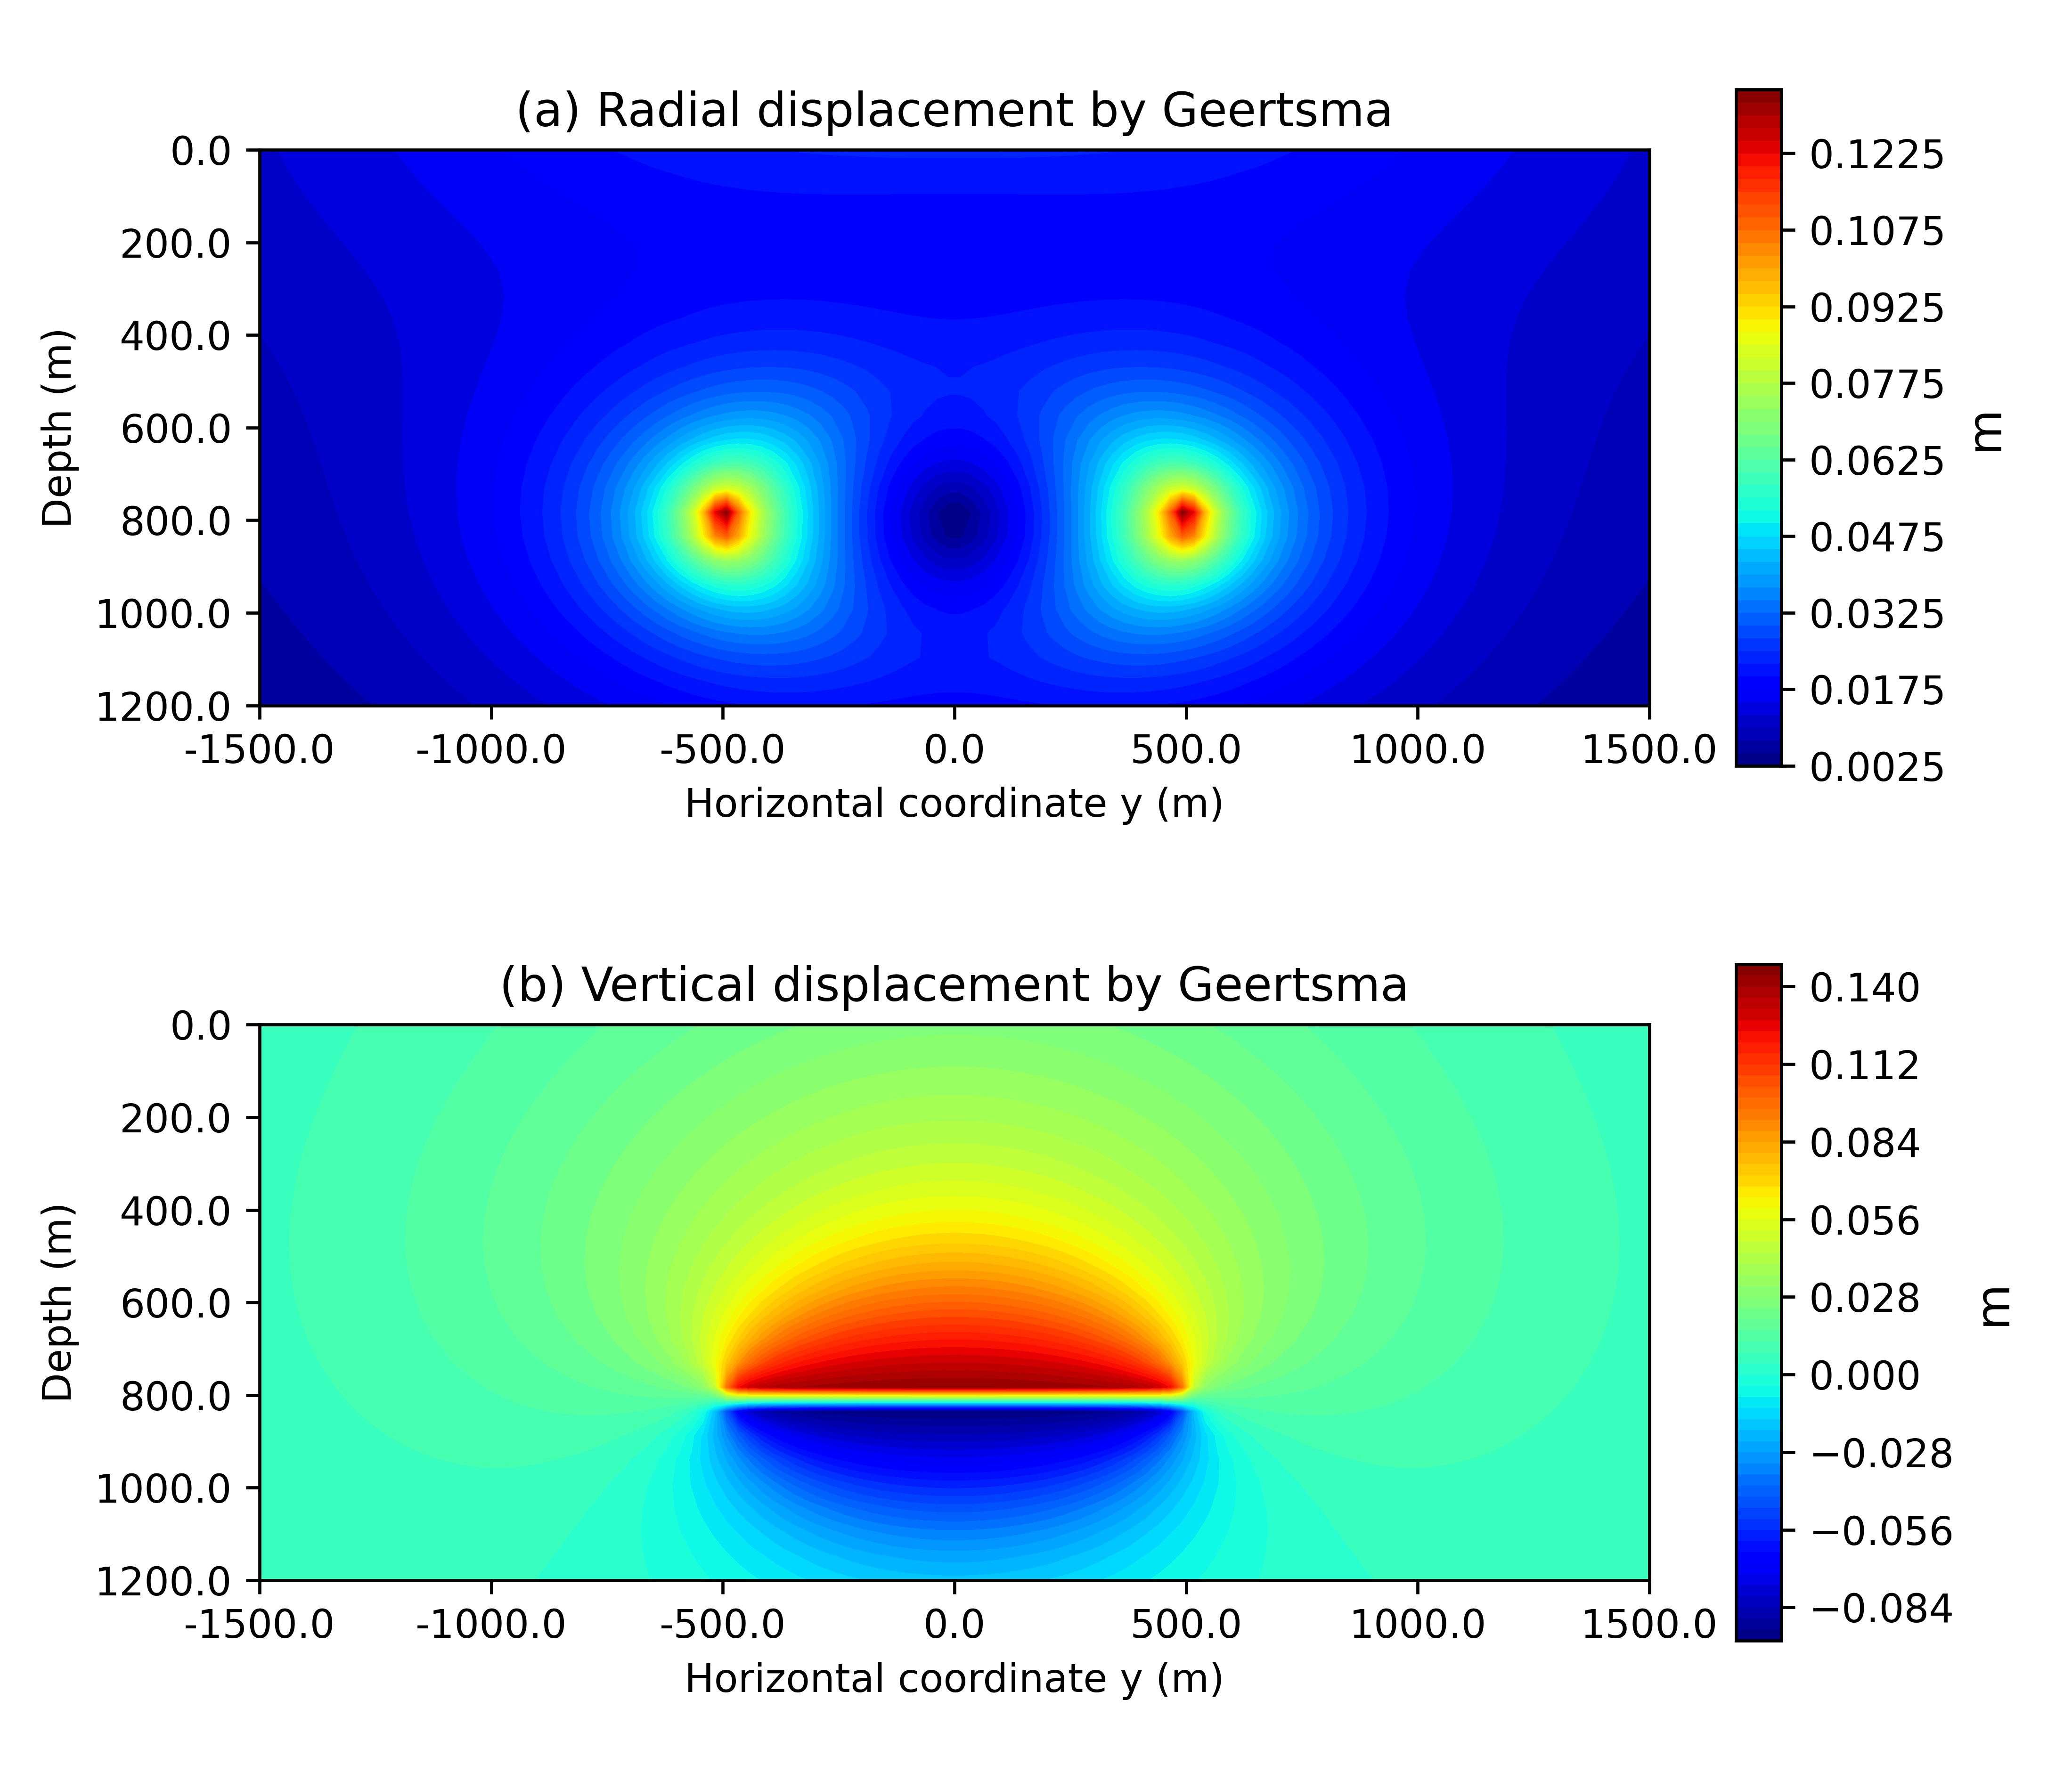
\includegraphics[scale=0.40]{figures/Figure_Displacement_Geertsma.png}
    \caption{Reservoir under uniform depletion: (a) Radial displacement and (b) vertical displacement using 
    Geertsma’s method \citep{Geertsma73}  considering an elastic homogeneous cylindrical reservoir under 
    uniform depletion \citep{Fjaer08}.}
	\label{fig:displacement_Geertsma}
\end{figure} 
\begin{figure}[h]
    \centering
    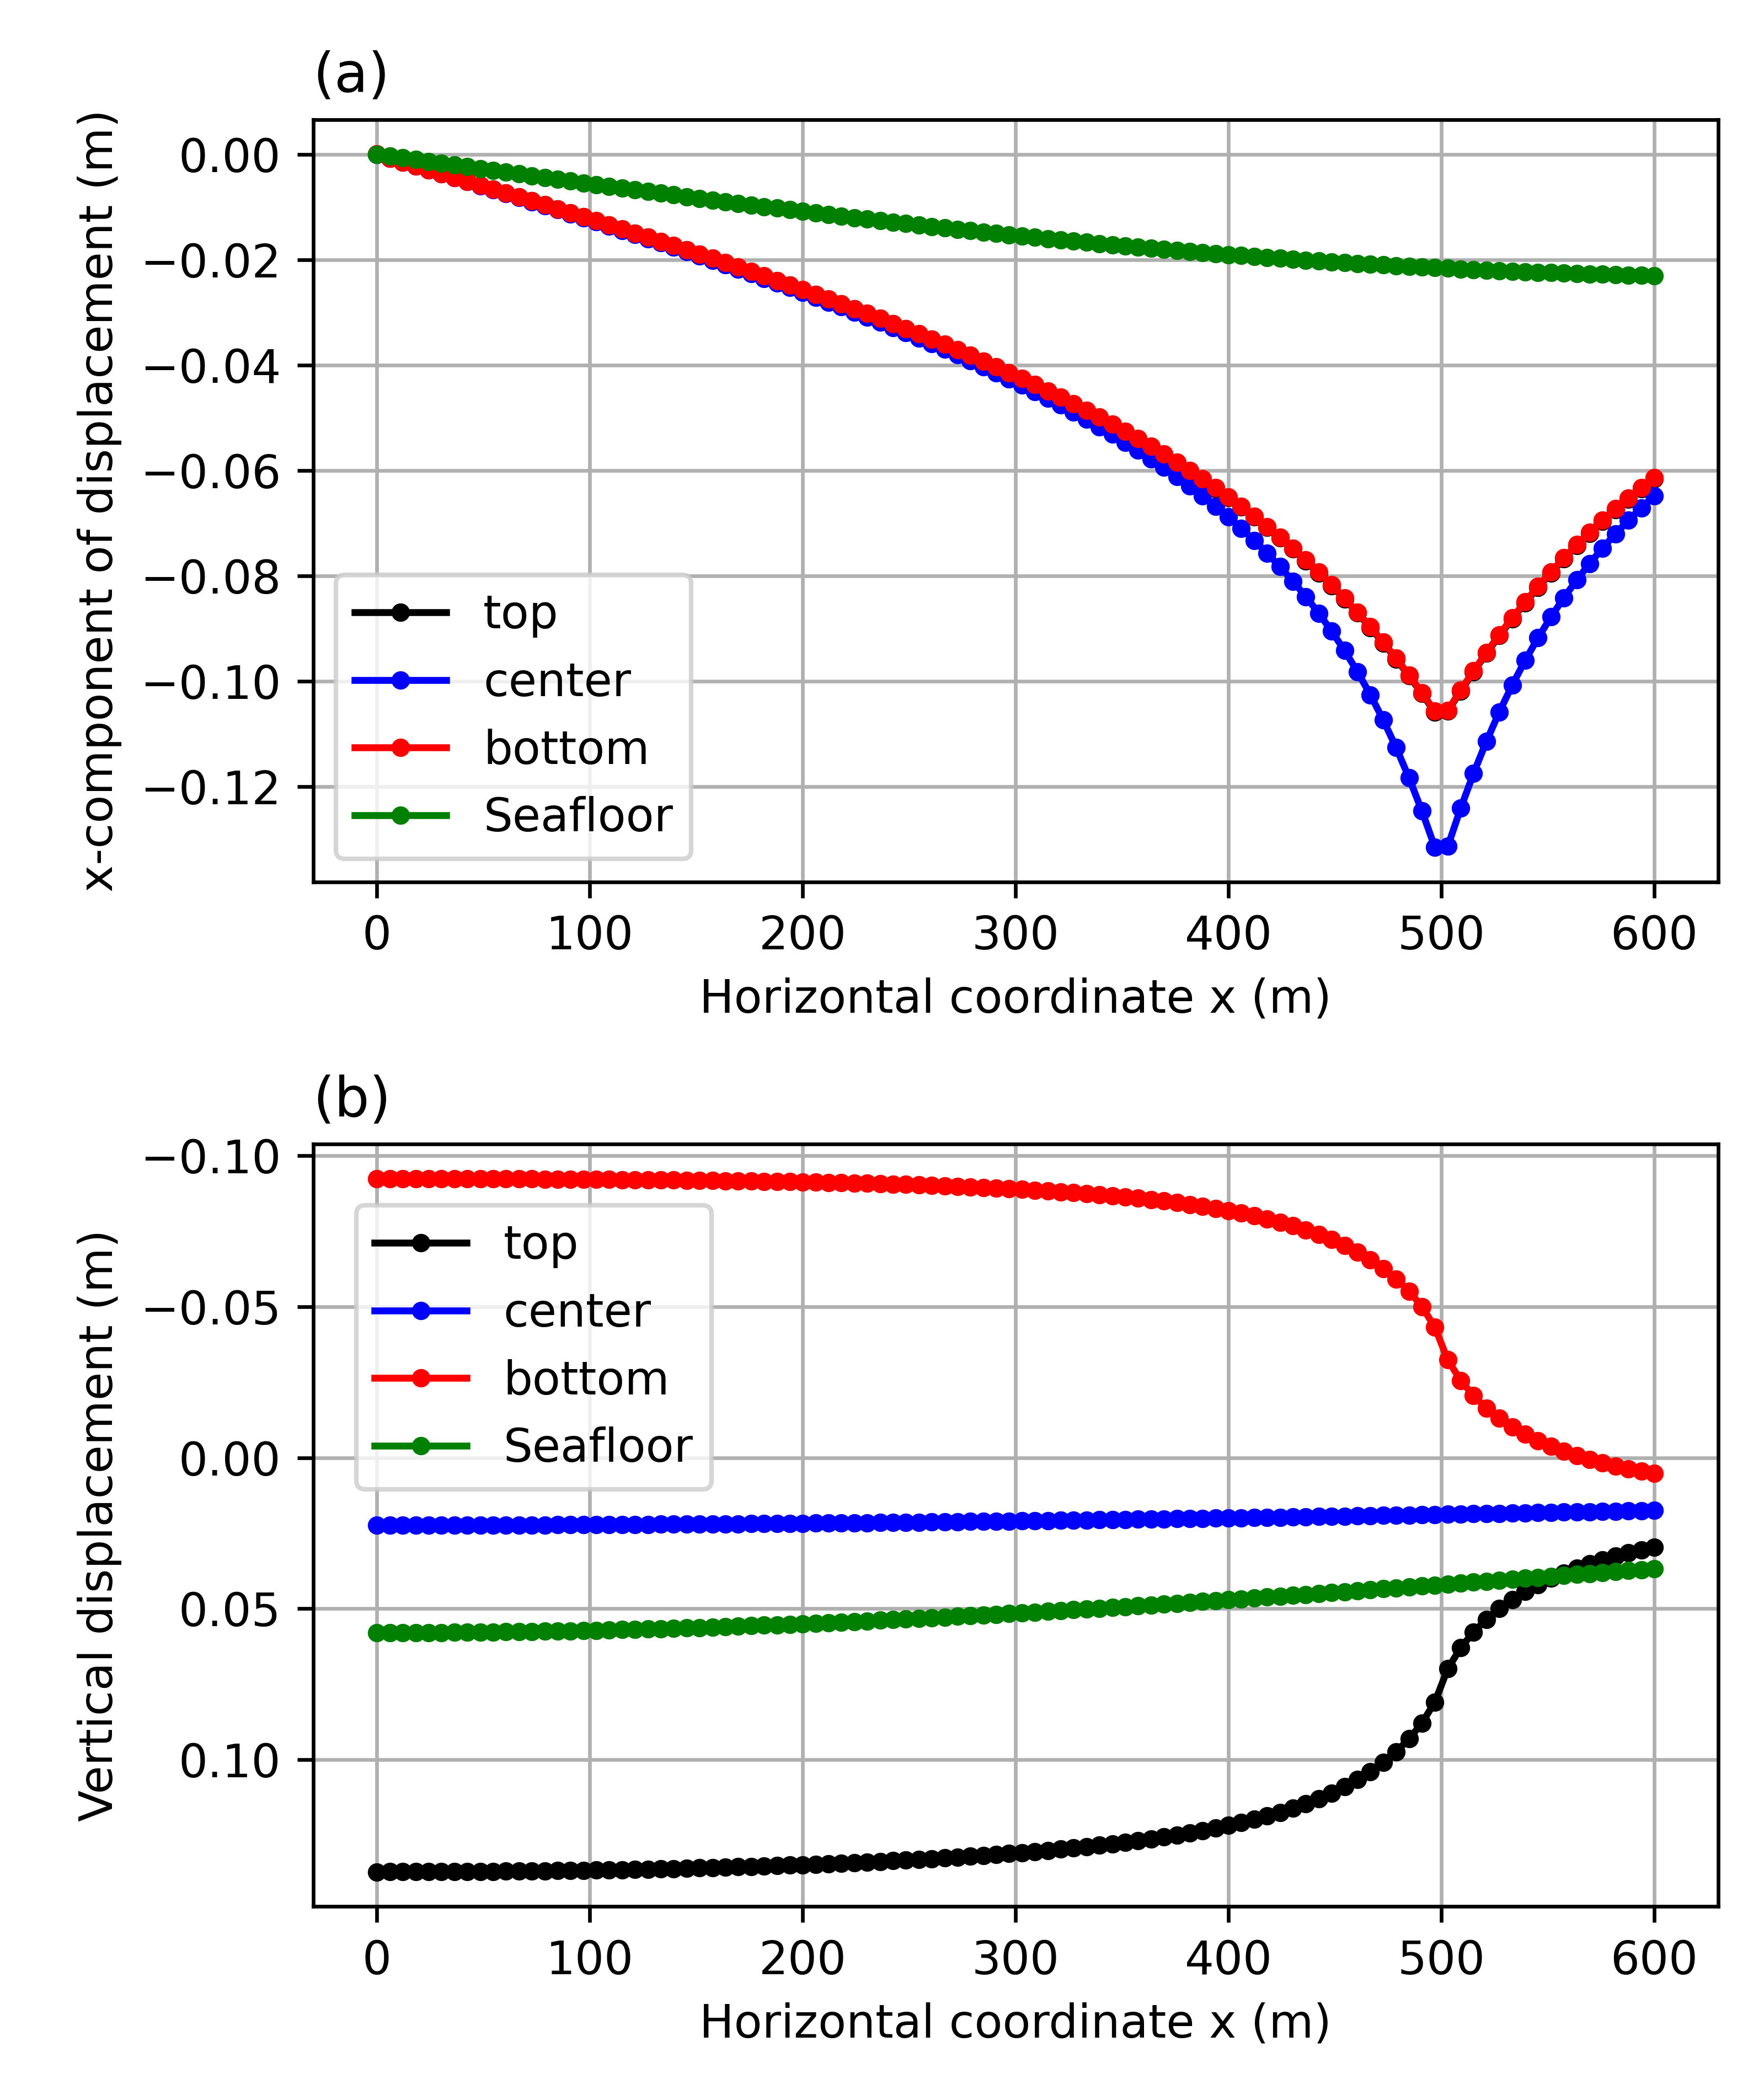
\includegraphics[scale=0.40]{figures/Figure_Displacement_z_levels.png}
    \caption{Reservoir under uniform depletion: (a) horizontal $x$-component displacement and (b) vertical 
	displacement by our methodology that uses the closed expressions of the volume integrations (equations 
	\ref{eq:u_til_alpha} and \ref{eq:u_til_z}), whose closed solutions are given by equations \ref{dx1}--\ref{dzz2}.
	These displacements are calculated along the $x$-axis, at $y = 0$ m and $z$ located at the depths of:  
	seafloor ($z = 0$ m), reservoir top ($z = 750$ m), reservoir center ($z = 800$ m) 	and reservoir bottom ($z = 850$ m).}
	\label{fig:displacement_z_levels}
\end{figure} 
%\vspace{0.0cm}
\begin{figure}[!h]
    \centering
    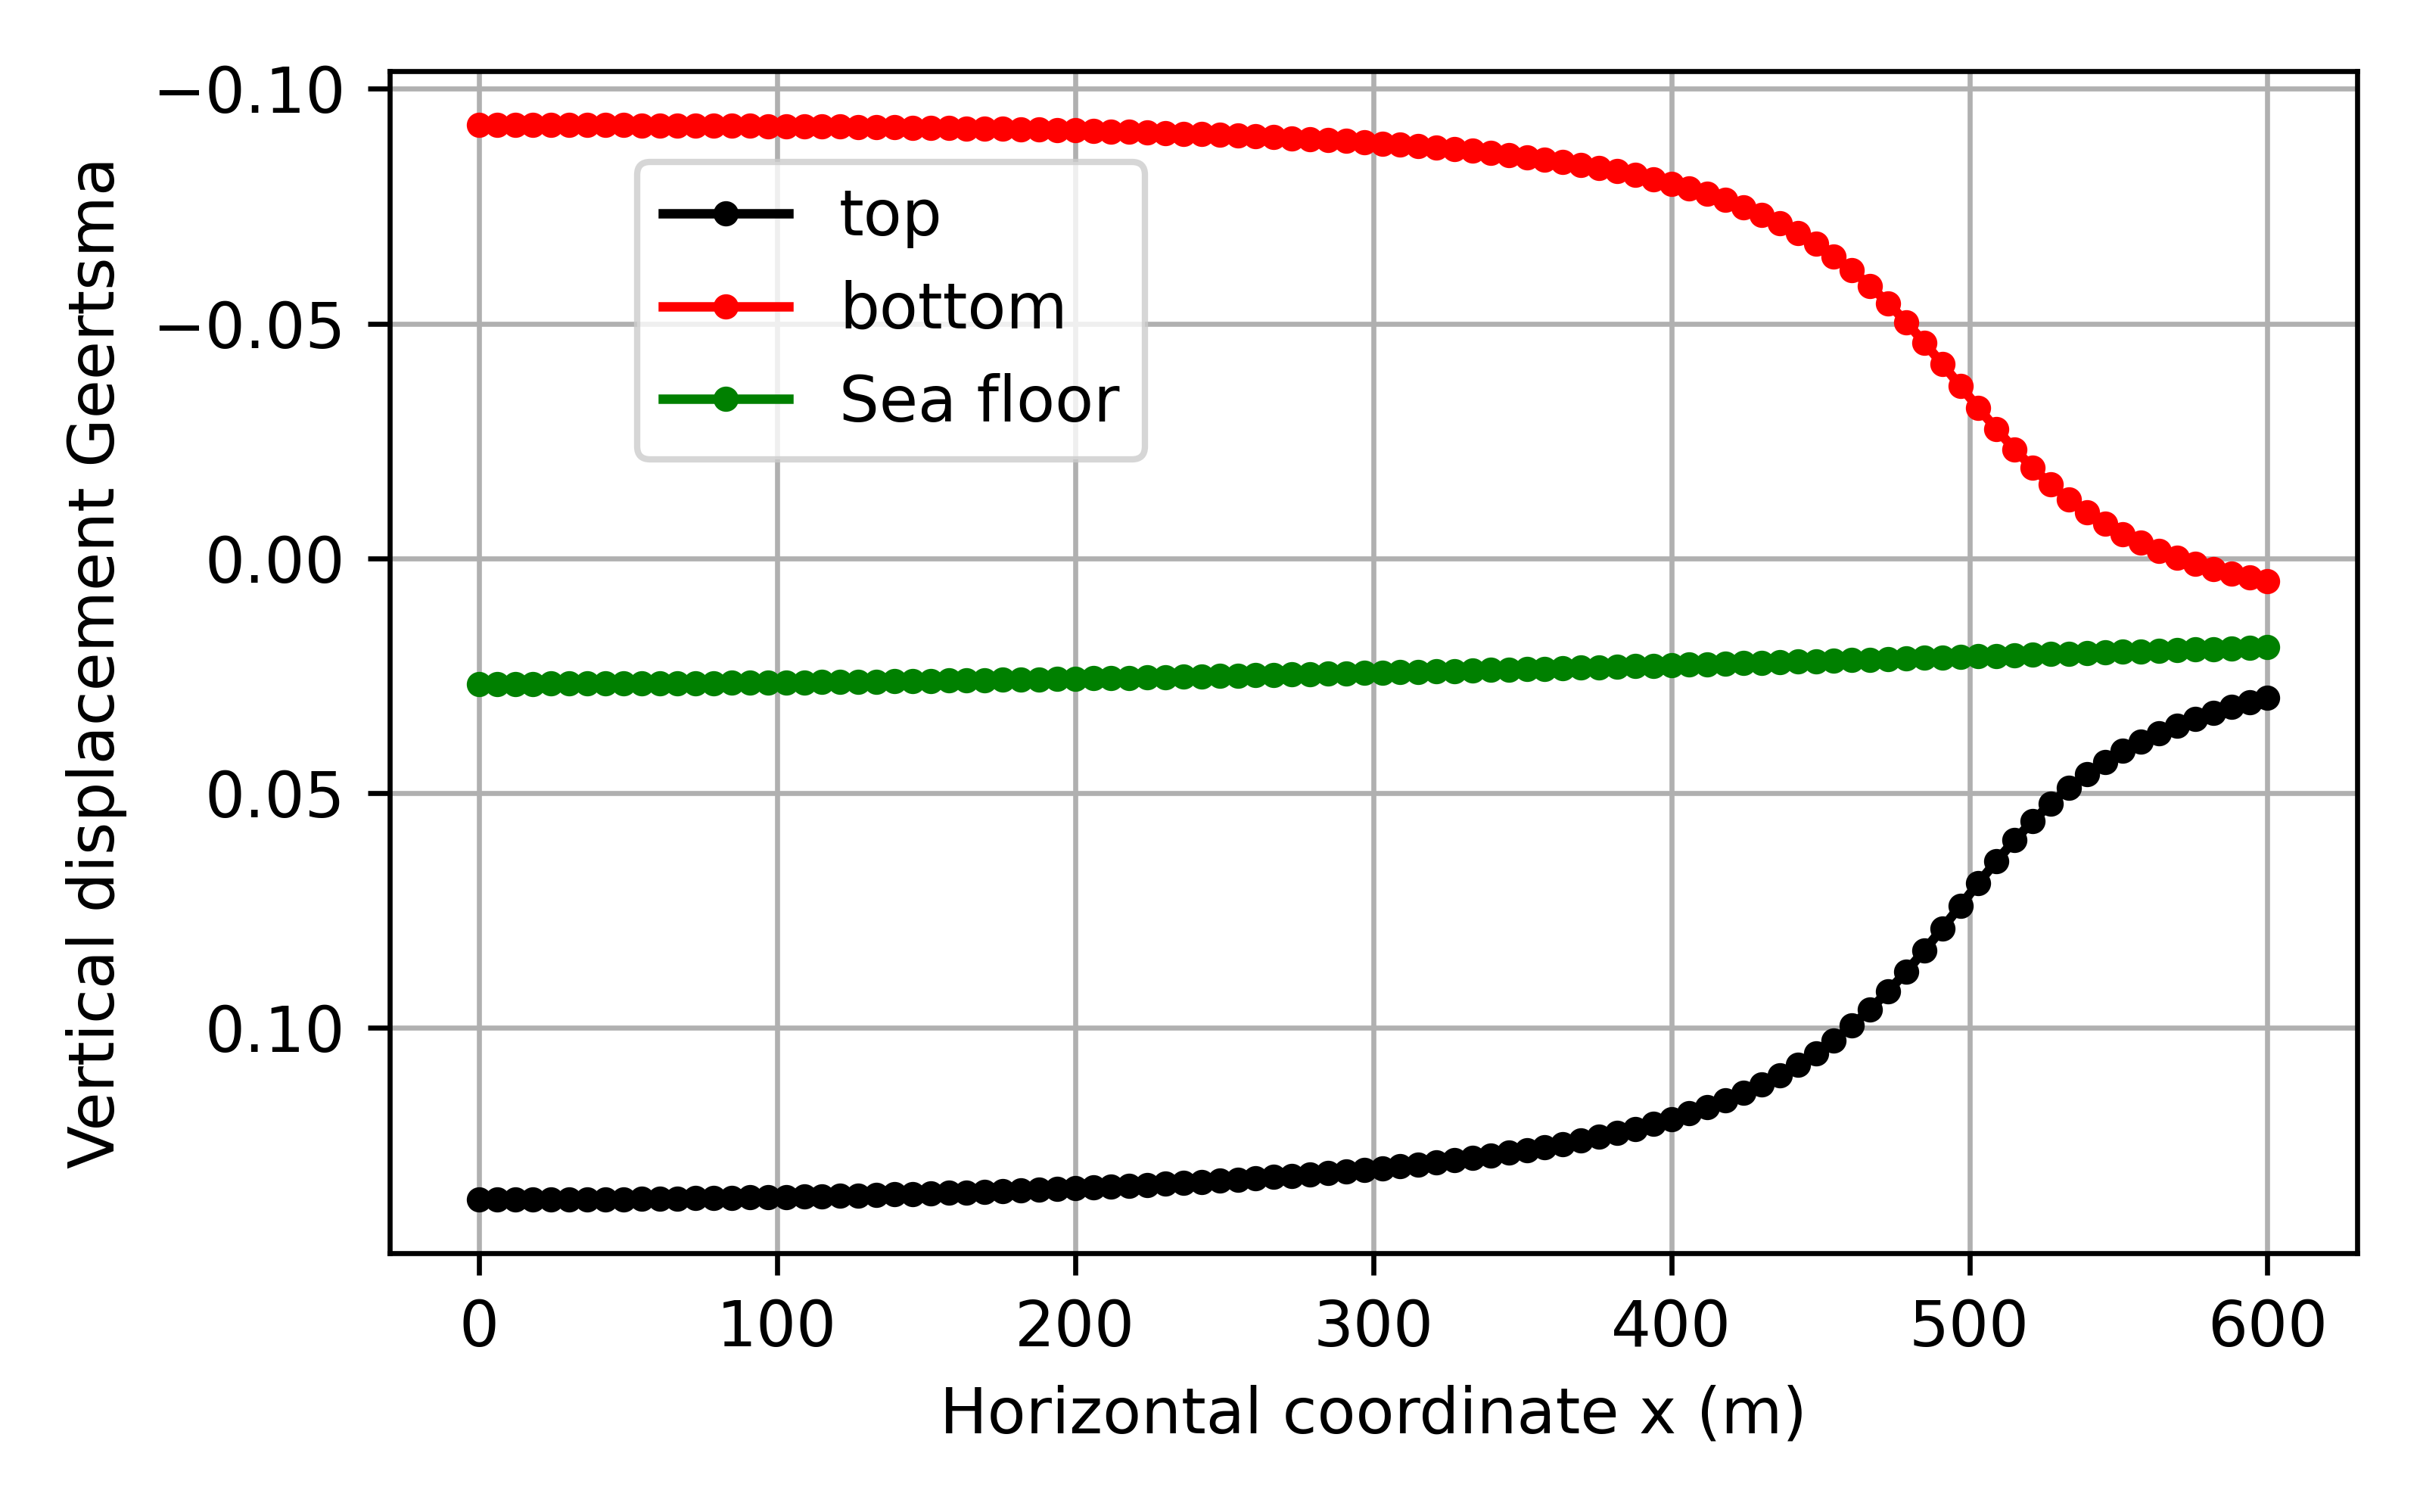
\includegraphics[scale=0.40]{figures/Figure_Displacement_z_levels_Geertsma.png}
    \caption{Reservoir under uniform depletion: vertical displacement using Geertsma’s method 
    \citep{Geertsma73}  
	considering an elastic homogeneous cylindrical reservoir under uniform depletion \citep{Fjaer08}.
	The displacement is calculated along the x-axis, at $y = 0$ m and $z$ located at the depths of:  seafloor 
	($z = 0$ m), reservoir top ($z = 750$ m), and reservoir bottom ($z = 850$ m).}
	\label{fig:displacement_z_levels_Geertsma}
\end{figure} 
%\vspace{-0.5cm}
\begin{figure*}[!t]
    \centering
    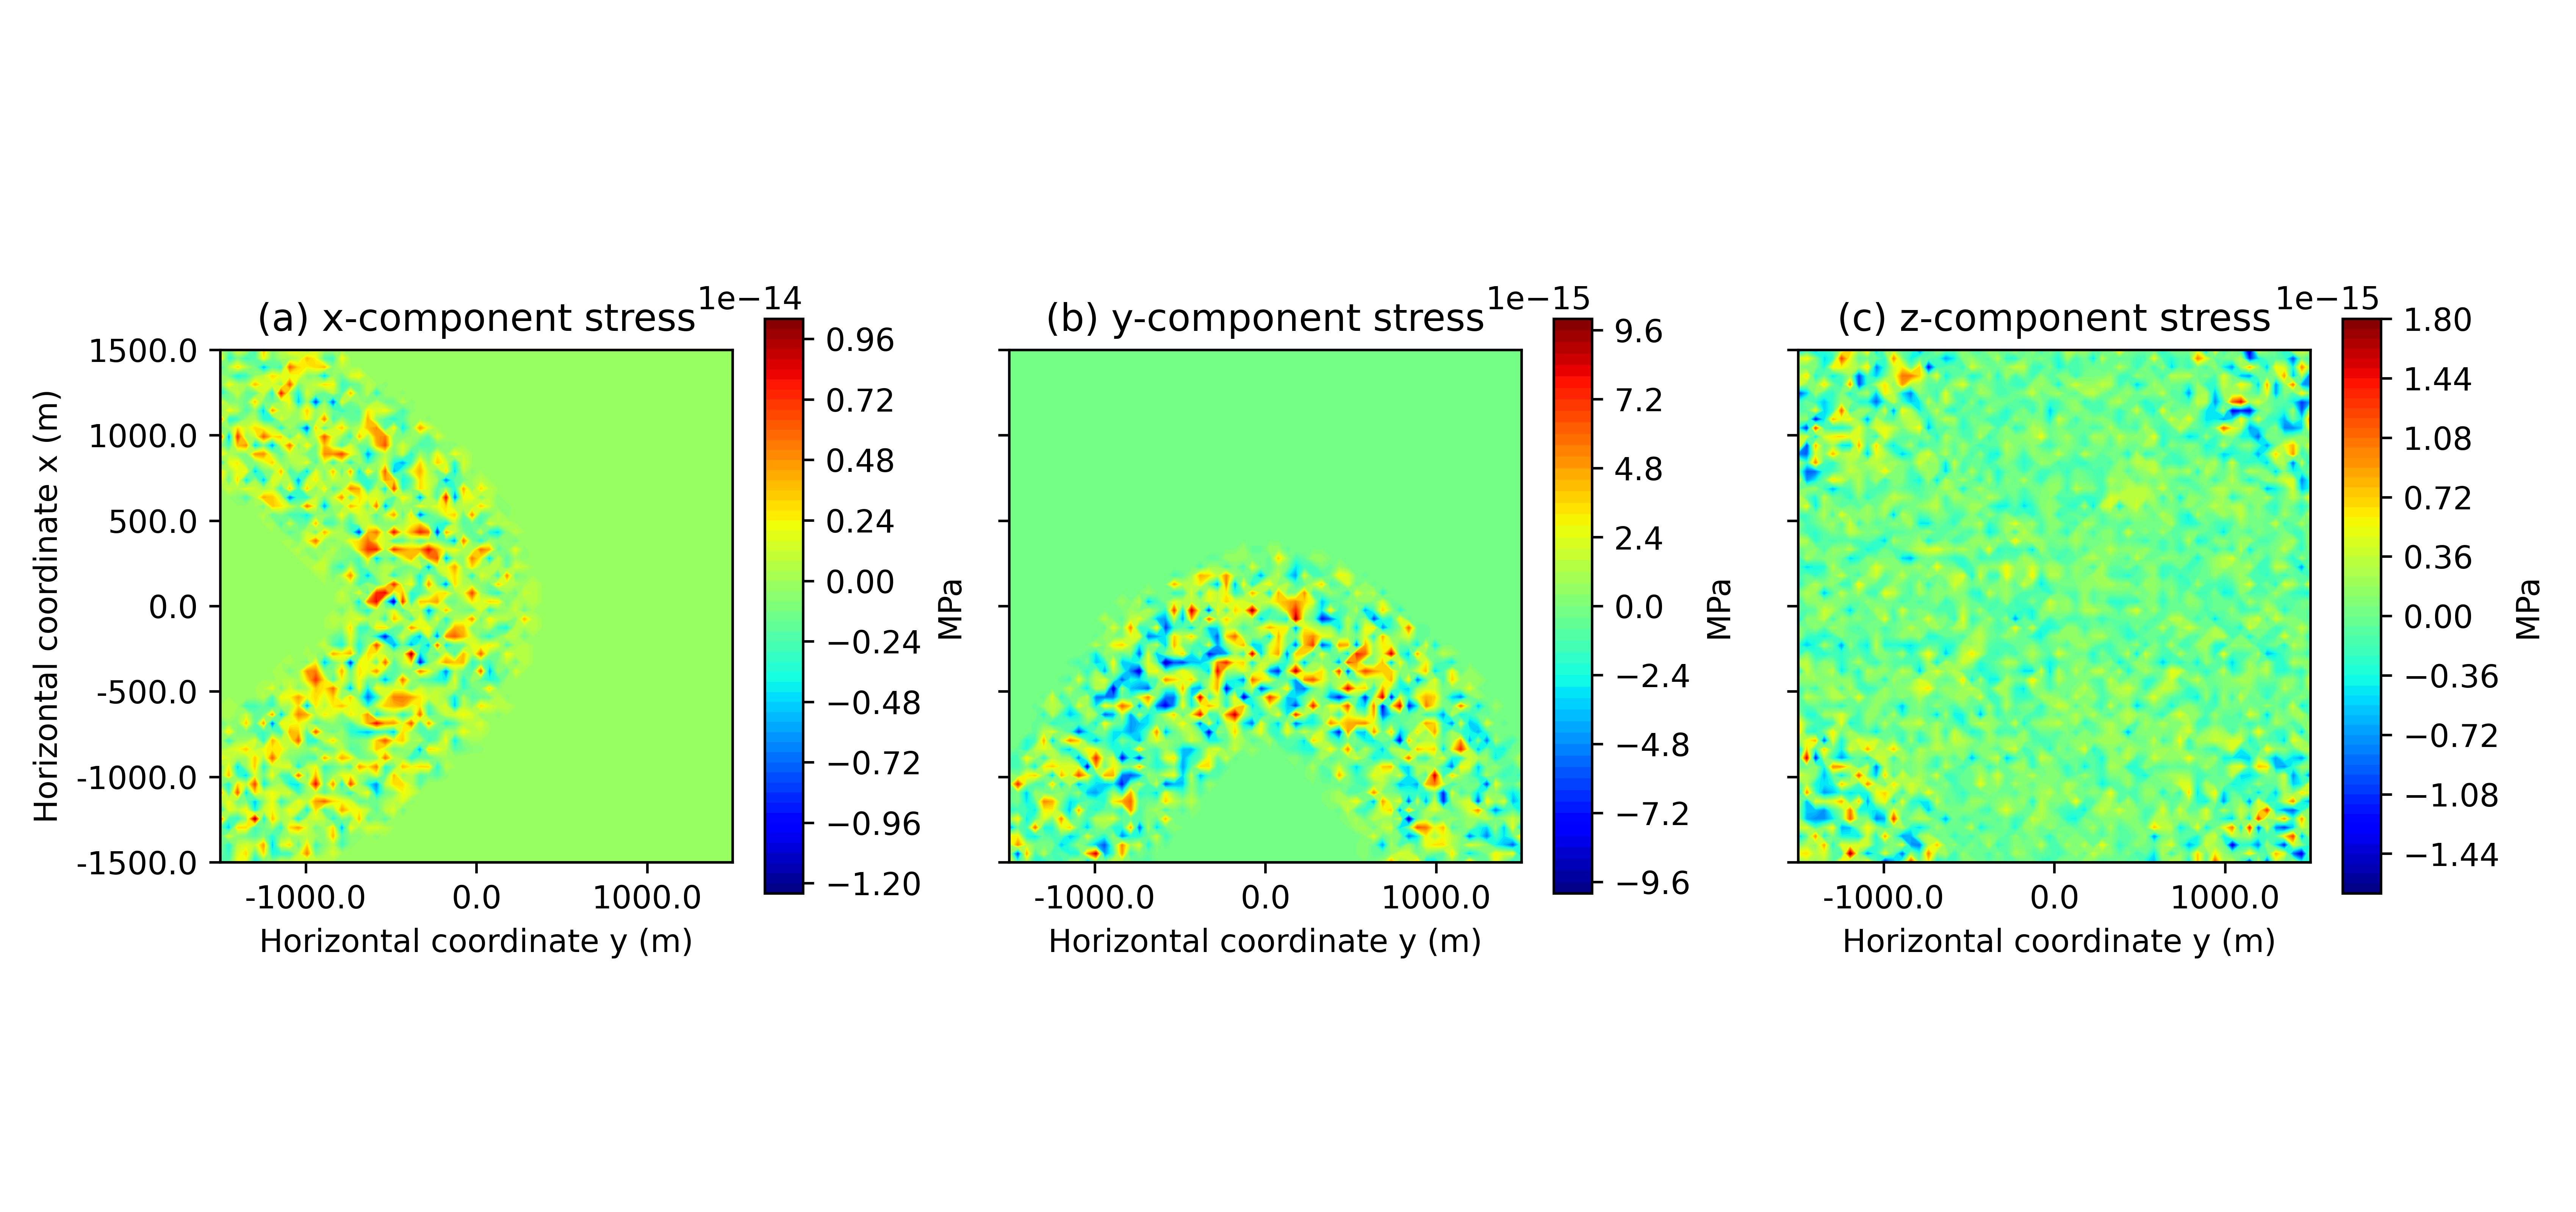
\includegraphics[width=\textwidth]{figures/Figure_Null_stress.png}
    \vspace{-2cm}
    \caption{Reservoir under uniform depletion: (a) $x-$, (b) $y-$, and 
    (c) $z-$components of the stress at the free surface. 
	The horizontal and vertical stresses are calculated by using 
	the full volume integrations (equations \ref{eq:stress_til_alpha} 
	and \ref{eq:stress_til_z}),
	whose closed solutions are given by equations \ref{dxz1}--
	\ref{sz3}.}
	\label{fig:Null_stress}
\end{figure*} 


%\newpage
\vspace{0.5cm}
\noindent{\textbf{Reservoir with arbitrary geometry and under arbitrary pressure changes}}
%\subsection*{Reservoir with arbitrary geometry and under arbitrary pressure changes}
%\vspace{-0.5cm}

In this numerical application, the reservoir model is a simplification of a realistic reservoir located in a production oil field in offshore Brazil.
The entire reservoir model comprises dimensions of 14 km in the north-axis, 13 km in the
east-axis, and 0.6 km in the down-axis. 
The depths to the top and bottom of the reservoir model are 2,712 m and 3,312 m, respectively. 
The components of the displacements are calculated at 0 m deep, 
on a regular grid of 100 $\times$ 80  observation points along the north- and east-directions, respectively. 
We  discretized the reservoir  along the $x-$, $y-$ and $z-$ directions into an $14 \times 13 \times 2$ grid of prisms.
The Young’s modulus is  3300 (in MPa), the Poisson's coefficient is 0.25, and
the uniaxial compaction coefficient $C_{m}$  (equation \ref{eq:Cm}) is $2.2525 \: 10^{-4}$
$\textrm{ MPa}^{-1}$.
Figure \ref{fig:pressure_complex_reservoir} shows the pore pressure distribution of the reservoir whose pressures vary from $0$ to $-0.72$ MPa.
Figure \ref{fig:displacement_complex_reservoir} shows cross-sections at $x  = 8$ km of the horizontal and vertical displacements, calculated in the whole reservoir by using our methodology.
Figure \ref{fig:Null_stress_complex_reservoir} shows the  null stress through the free surface 
due to reservoir shown in Figure \ref{fig:pressure_complex_reservoir}.
%The reservoir (Figure \ref{fig:pressure_complex_reservoir}) yields null stress (not shown) at the free surface 
\begin{figure}[h]
    \centering
    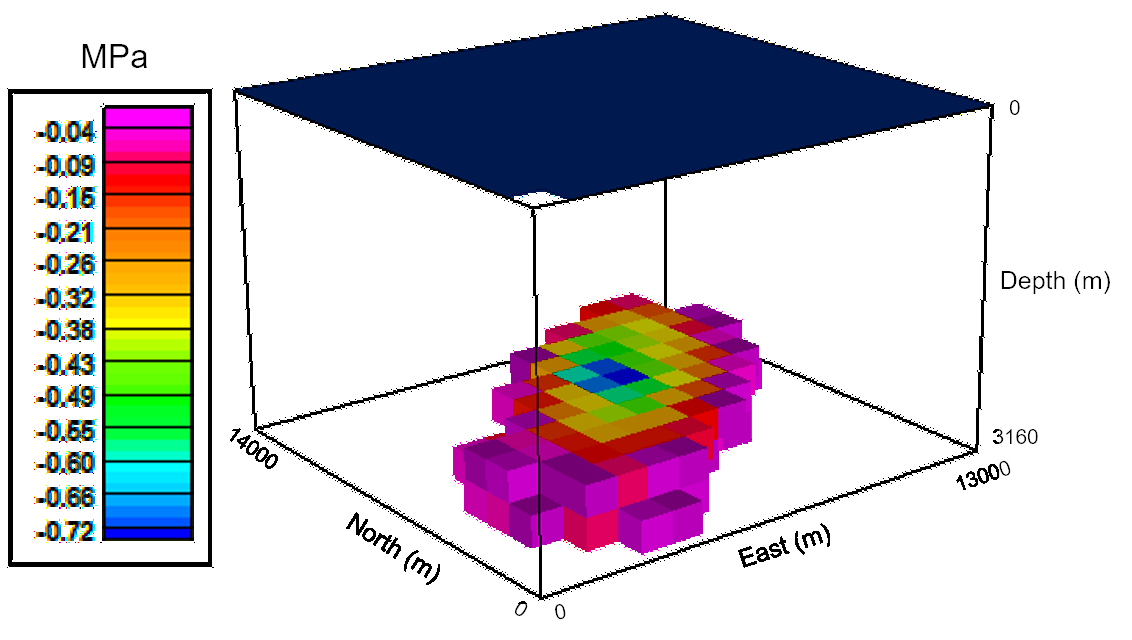
\includegraphics[scale=0.40]{figures/Figure_Pressure_complex_reservoir.png}
    \caption{Reservoir with arbitrary geometry and under arbitrary pressure changes: 3D perspective view of 
    the pore pressure distribution based on a reservoir located in a production oil field in offshore Brazil.}
	\label{fig:pressure_complex_reservoir}
\end{figure} 
\begin{figure}[t]
    \centering
    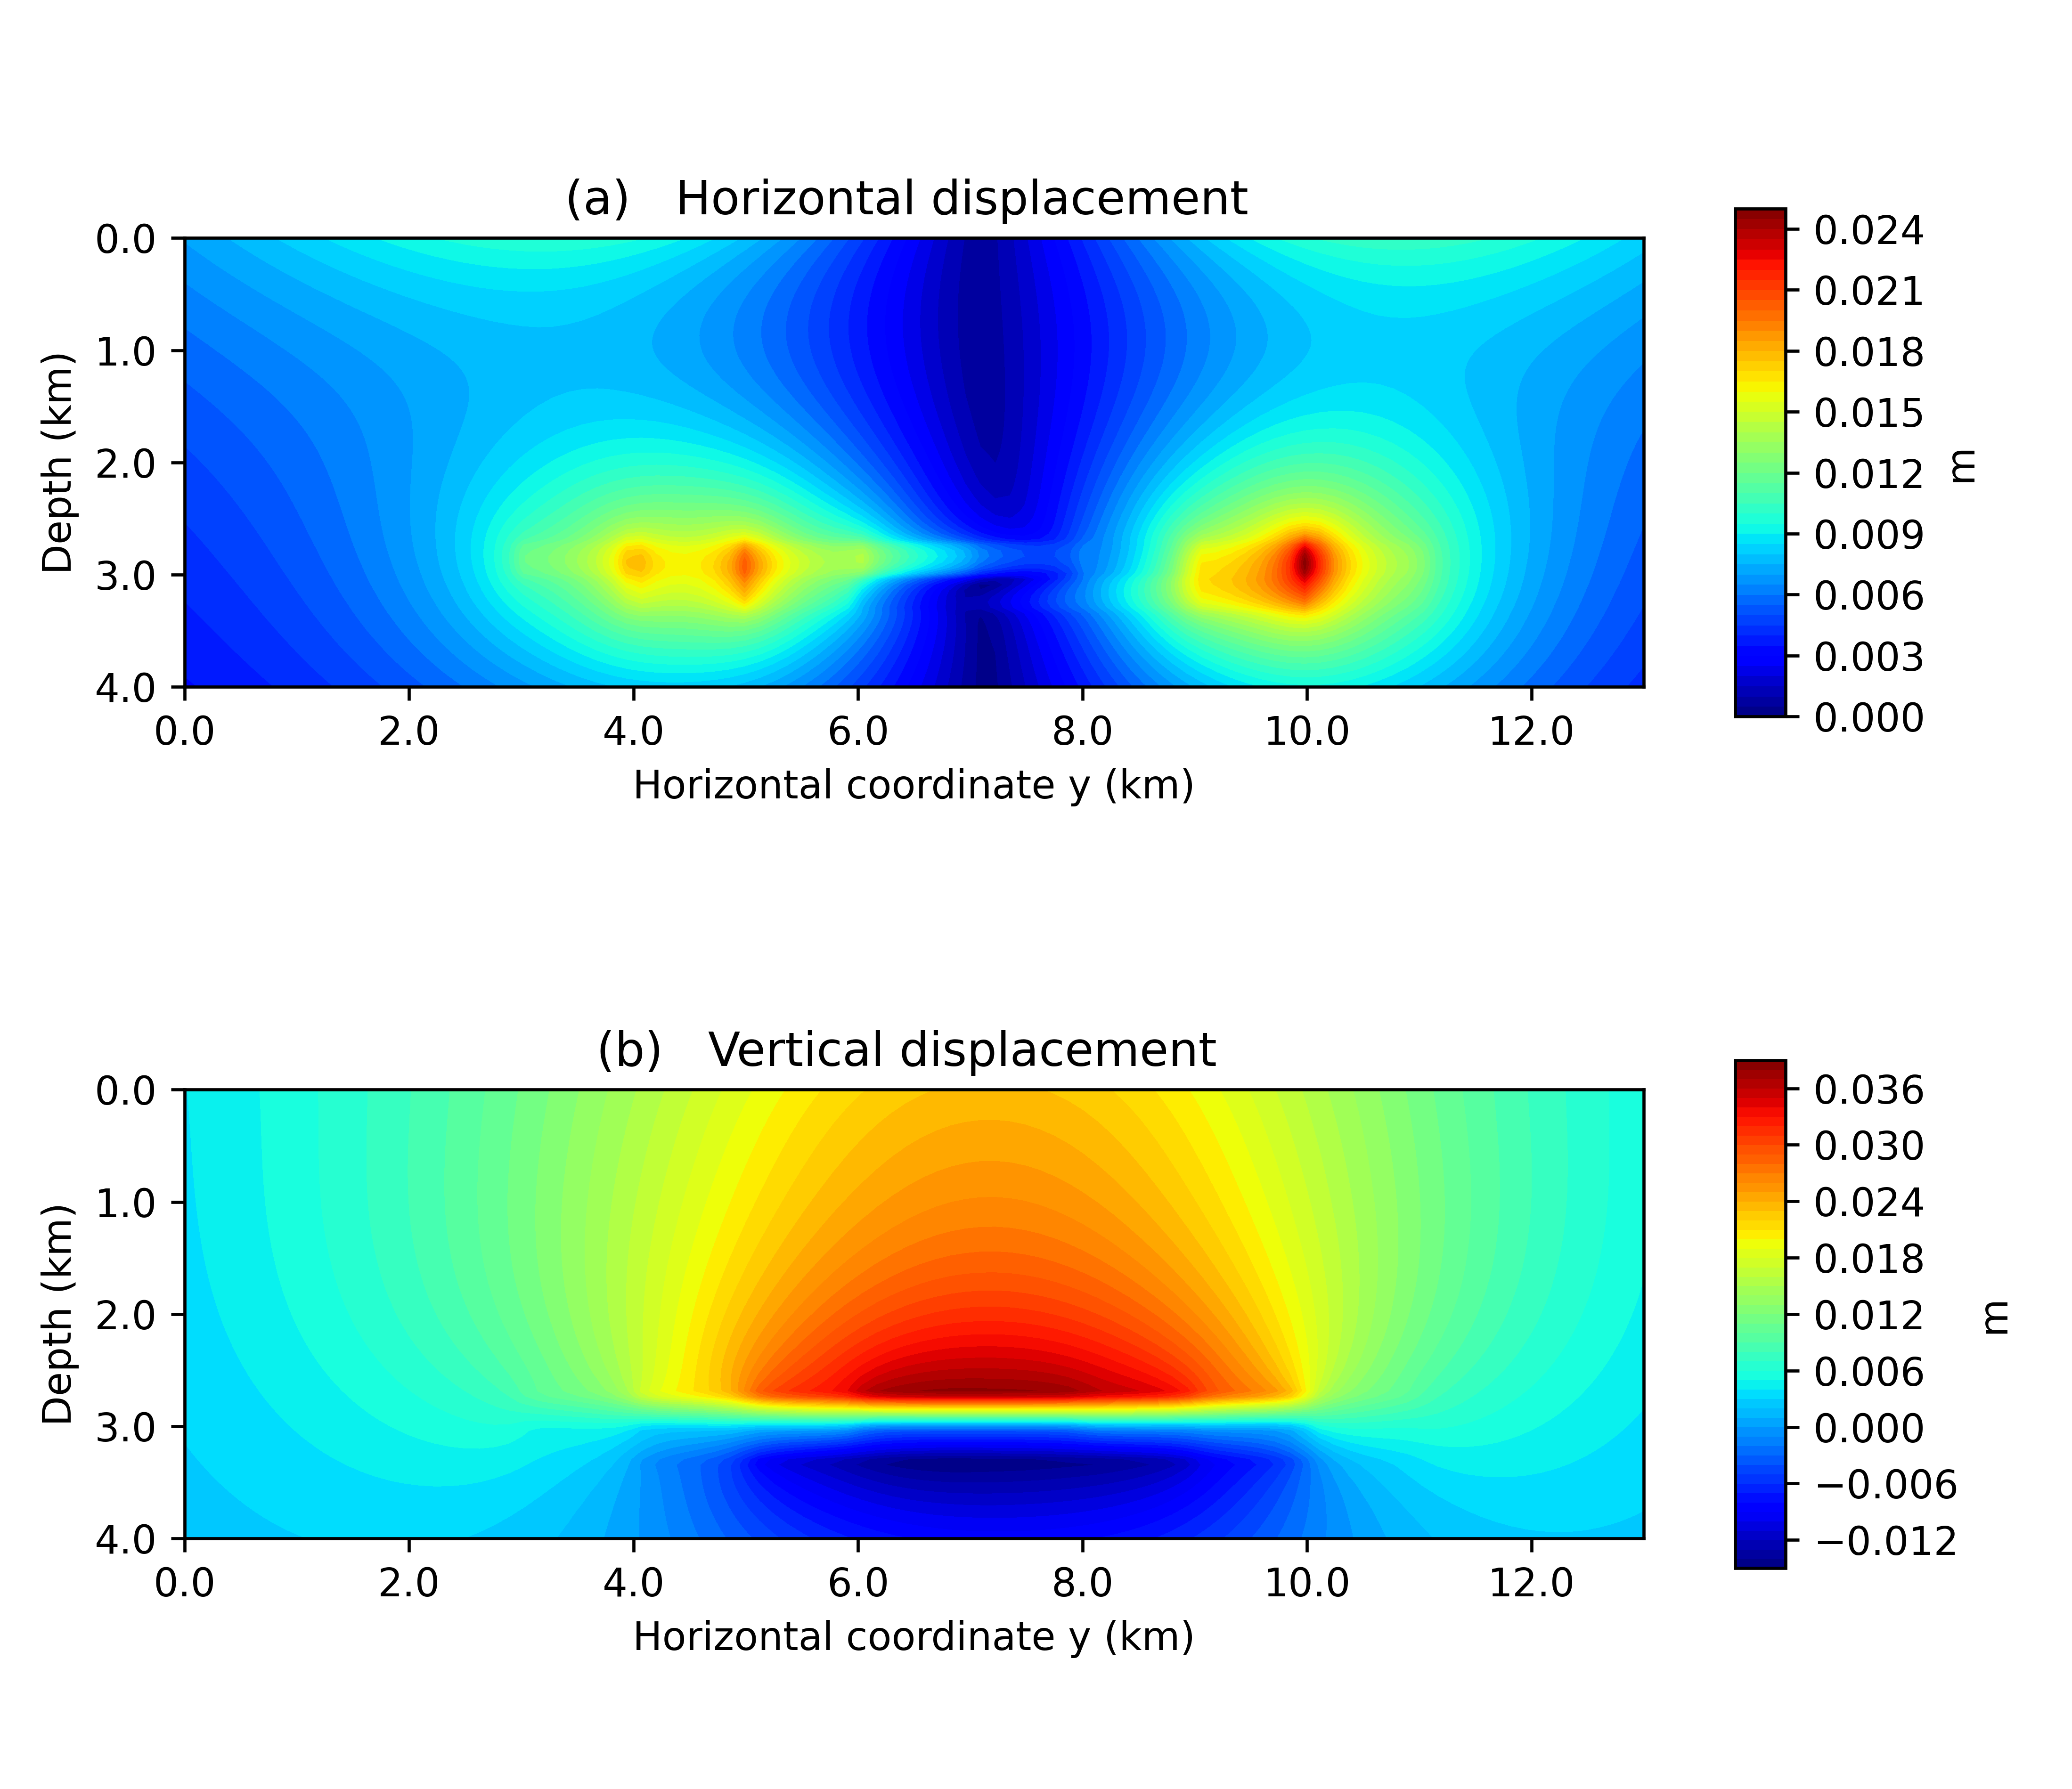
\includegraphics[scale=0.40]{figures/Figure_Displacement_complex_reservoir.png}
    \vspace{-0.5cm}
    \caption{Reservoir with arbitrary geometry and under arbitrary pressure changes: 
    (a) horizontal displacement (equation \ref{eq:horizontal_displacement}) and (b) vertical displacement 
    (equation \ref{eq:u_til_z}) by our methodology that uses the closed expressions of the volume integrations 
	(equations \ref{eq:u_til_alpha} and \ref{eq:u_til_z}), whose closed solutions are given by equations 
	\ref{dx1}--\ref{dzz2}.}
	\label{fig:displacement_complex_reservoir}
\end{figure}


%\vspace{-1.0cm}
\section*{Conclusion}
%\vspace{-0.5cm}
Grounded on the similarity between the gravitational potential produced by a volume source under a density variation and the displacement field produced by a volume source in a half-space under a pressure variation, we have presented an alternative solution for the displacement and stress fields outside and inside of a 3D right rectangular prism with constant pressure change. 
Our solution is obtained by integrating the well-known nucleus-of-strain solution over the volume of the prism. 
We also use our solution to approximate the displacement and stress fields due to a reservoir compaction with arbitrary geometry and under non-uniform  pressure distribution.
Our approach consists in approximating the reservoir 3D pressure distribution through a piecewise constant function defined on a user-specified grid of 3D prisms juxtaposed in the $x-$, $y-$ and $z-$directions.
The sum of the displacements(stresses) produced by the prisms is the resultant displacement(stress) field due to the whole reservoir.
Our expressions are valid either outside or inside the prisms.
We have demonstrated the use of these expressions by applying them to calculate the displacement and stress fields due to cylindrical reservoirs with uniform and non-uniform pressure distributions and to a reservoir model of a production oil field in offshore Brazil.
All the numerical applications produced null stress fields  at the free surface showing that the condition of null tractions at the free surface has been met. 
%\footnote{Note for editor and reviewers: Following the concept of reproducible science which requires the
%open-source code, the computer codes, supporting documentation and numerical applications showing the results %will be freely available through online repositories at the end of the review process.}

\section*{Acknowledgments}
We thank the editor George Sand L.A. de Fran\c{c}a and the reviewers for their criticisms and suggestions.
Barbosa V.C.F. and Oliveira Jr V.C.  were supported by fellowships from  the Brazilian research agencies: CNPq (grants 309624/2021-5 and 315768/2020-7) and FAPERJ (grants E-26/202.582/2019 and E-26/202.729/2018). 
Arelaro A.D. and Borges F. thank PETROBRAS.

\section*{Code and data availability}
The current version of our code is freely distributed under the BSD 3-clause licence and it is available for download at Zenodo: \texttt{https://doi.org/10.5281/zenodo.4041984}. 
The latest development version of our code can be freely downloaded from a repository on GitHub (\texttt{https://github.com/pinga-lab/DisReserv}). 
Instructions for running  the current version of our code are also provided on the repository.
The code is still being improved and we encourage the user to work with the latest development version. 
The code was developed as an open-source Python language (Python 3.7.x).
The numerical applications were produced in Jupyter Notebook. 
The data of the pore pressure distribution simulating a reservoir with arbitrary geometry and under arbitrary pressure changes
(\textit{realistic-model.pickle}) are available  in the  above-mentioned repositories.

\begin{figure*}[!t]
    \centering
    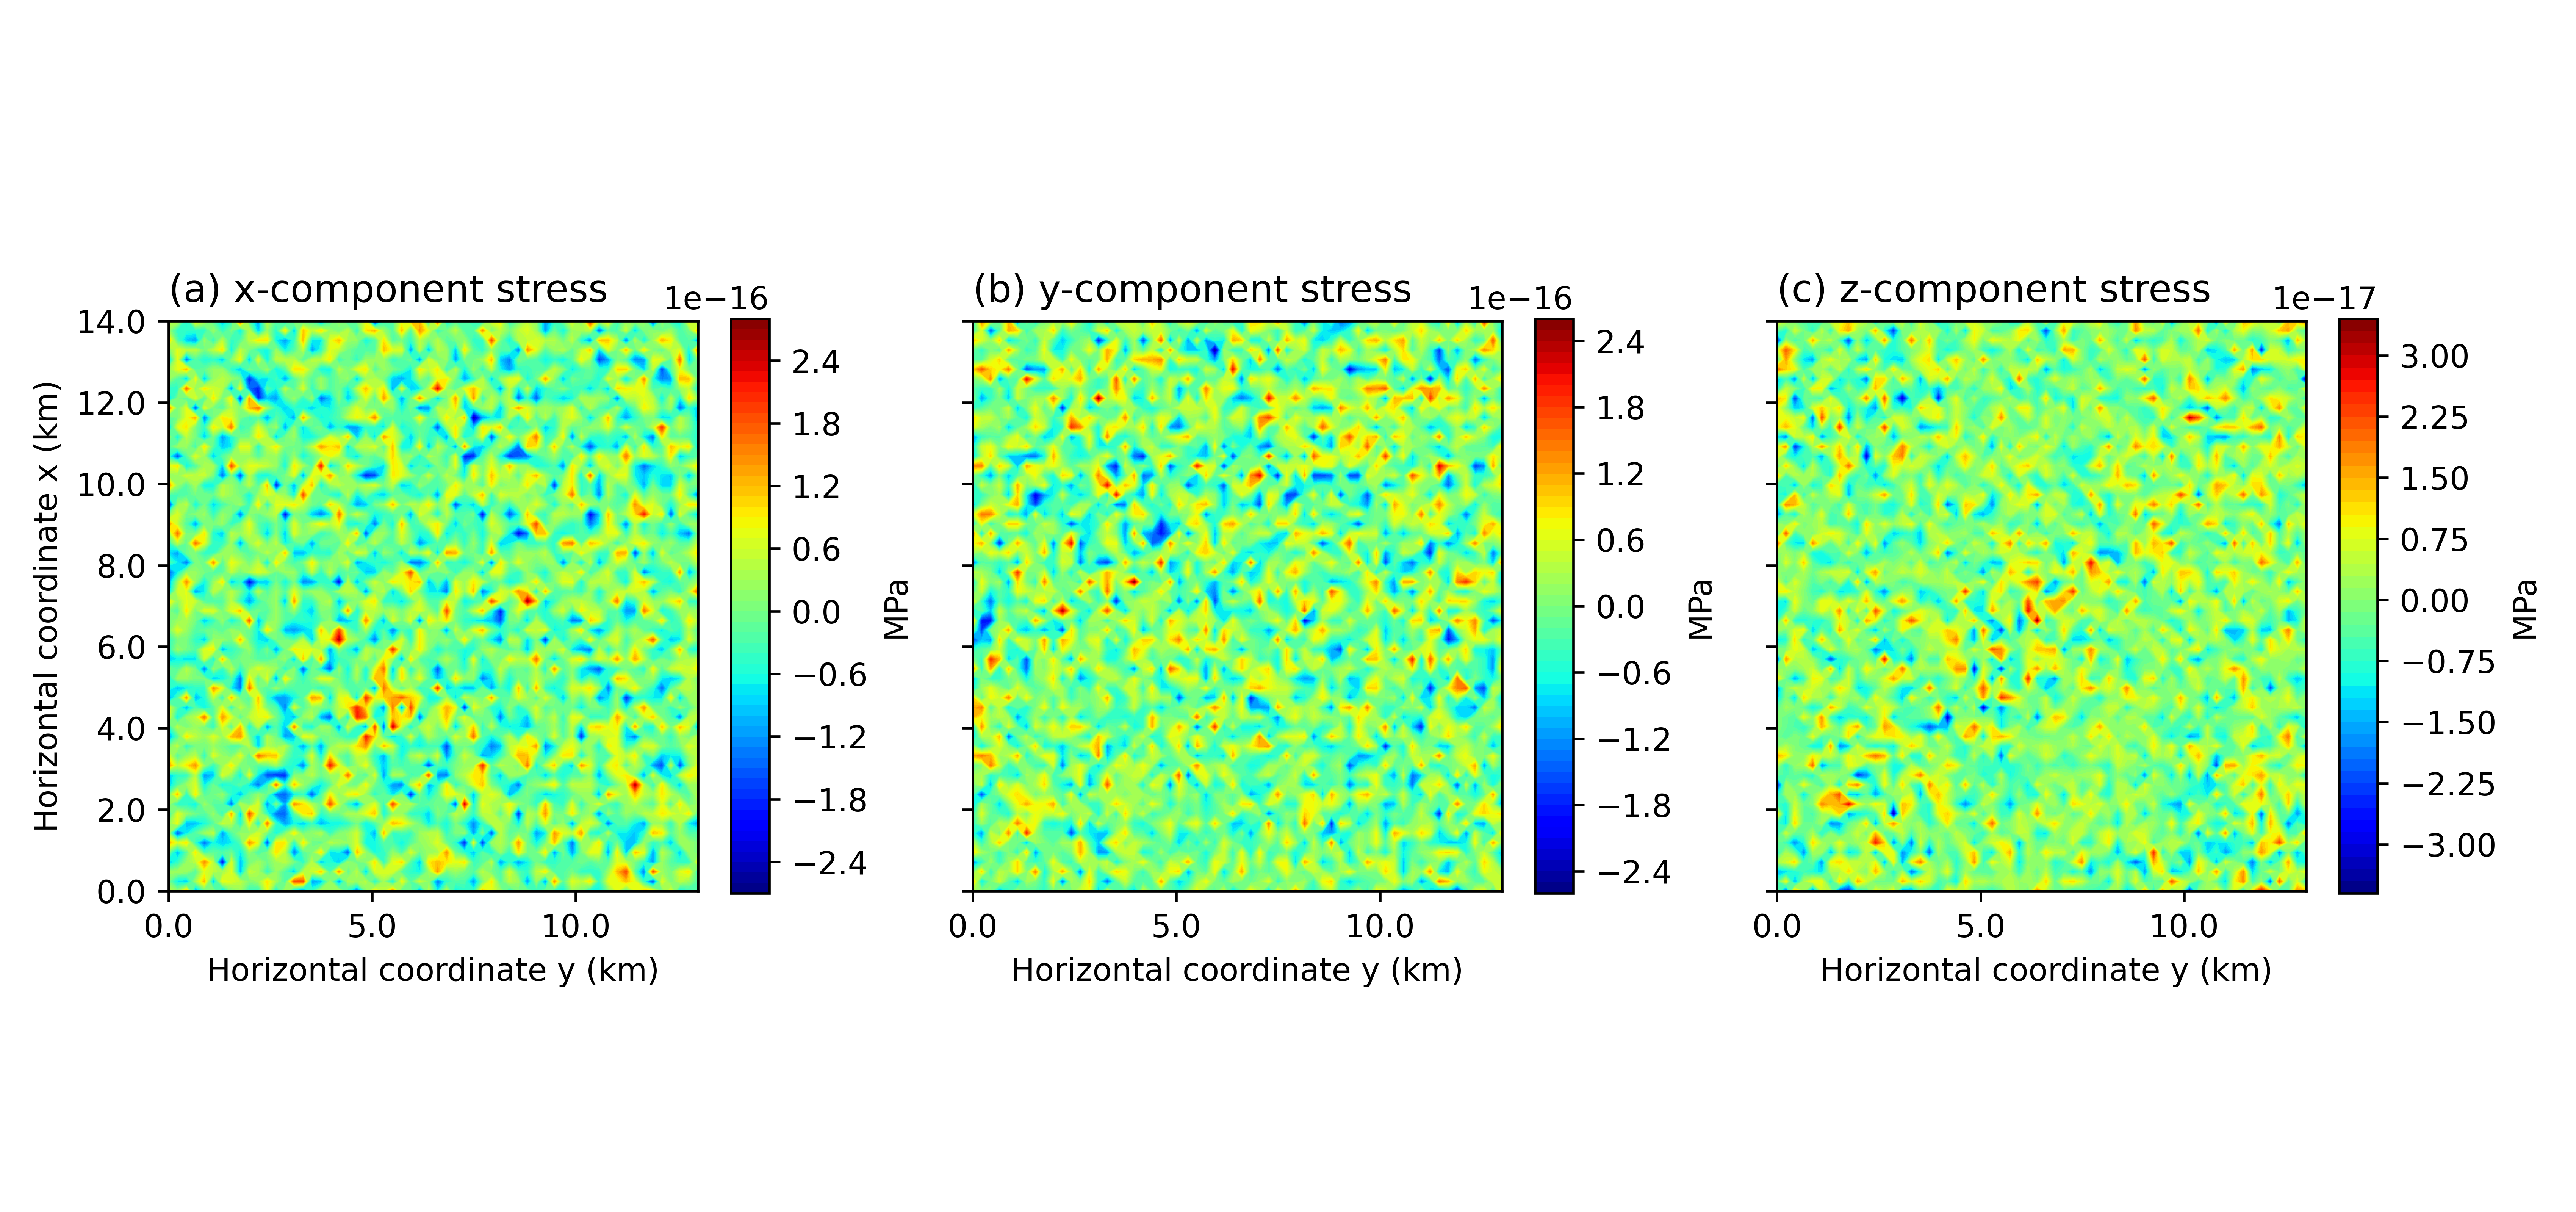
\includegraphics[width=\textwidth]{figures/Figure_Null_stress_complex_reservoir.png}
    \vspace{-2.0cm}
    \caption{Reservoir with arbitrary geometry and under arbitrary pressure changes: 
    (a) $x-$, (b) $y-$, and (c) $z-$components of the stress at the free surface.
	The horizontal and vertical stresses are calculated by using 
	the full volume integrations (equations \ref{eq:stress_til_alpha} and \ref{eq:stress_til_z}),
	whose closed solutions are given by equations \ref{dxz1}--\ref{sz3}.}
	\label{fig:Null_stress_complex_reservoir}
\end{figure*}

%%%%%%%%%%%%%%
\bibliographystyle{rbgf} 
\bibliography{references_RBGF}
%\bibliography{ref_teste}



\end{document}